%%%%%%%%%%%%%%%%%%%%%%%%%%%%%%%%%%%%%%%%%%%%%%%%%%%%%%%%%%%%%%%
%% HKUST Thesis LaTeX Template
%%
%% Check the project website for latest updates:
%% https://github.com/HKFoggyU/hkust-thesis
%%
%% Contributors:
%% https://github.com/HKFoggyU/hkust-thesis/graphs/contributors
%% 
%% License:
%% LaTeX Project Public License (version 1.3c)
%%
%%%%%%%%%%%%%%%%%%%%%%%%%%%%%%%%%%%%%%%%%%%%%%%%%%%%%%%%%%%%%%%

%% Pass options to loaded packages in `.cls` file:
% \PassOptionsToPackage{separate-uncertainty=true, separate-uncertainty-units=single}{siunitx}

%% The following option is to set hyperref colors for preview,
%% but commented by default for submission and printing
% \PassOptionsToPackage{colorlinks=true,urlcolor=blue,citecolor=red,anchorcolor=blue}{hyperref}

%% The following option is to display the full name of the authors.
%% It comes with the setting to display the full author names in the List of Publications
\PassOptionsToPackage{firstinits=false}{biblatex}

\documentclass[
  %customlatinfont = windows,
  %custombibstyle = nature,
  displaycommittee = false,
  blankpage = true,
]{hkustthesis}

\usepackage{float}
\usepackage{wasysym}
\usepackage[many]{tcolorbox}
\usepackage{tikz-cd}
\usetikzlibrary{tikzmark, calc}
\usepackage{tkz-euclide}
\usepackage{string-diagrams}
% \newcommand{\tikzmark}[1]{\tikz[overlay,remember picture] \node (#1) {};}

%% Thesis information
\hkustsetup {
  %% Please wrap the items with {}.
  %% If one item is not applicable, just leave it {}.
  %% Please do not leave any blank lines without {}.
  info = {
    degree        = {mphil},  %% phd / mphil
    title         = {Algebraic Logic\texorpdfstring{\\}{}for Deep Learning},
    keywords      = {algebraic logic, deep learning, artificial intelligence},
    author        = {YKY},
    school        = {Some Univ in Canada},
    department    = {Department of Maths},
    program       = {Applied Mathematics},
    major         = {},
    supervisor    = {Prof. Who},
    %% Co-supervisor; leave it {} if not available
    co-supervisor = {Prof. Who Else},
    submit-month  = {August 2024},      % <month year>
    submit-date   = {13 August 2024},   % <date month year>
    defend-date   = {8 March 2024},     % <date month year>
    depthead      = {Prof. Someone, Head of Department},
    %% reviewers only for some departments, like ECE
    reviewer      = {Prof. AAA (Chairperson), 
                     Prof. BBB (Supervisor),
                     Prof. CCC (Co-Supervisor),
                     Prof. DDD,
                     Prof. EEE,
                     Prof. FFF},
    reviewerdept  = {Department of Electronic and Computer Engineering,
                     Department of ECE,
                     Department of ECE,
                     Department of ECE,
                     Department of ECE,
                     Department of Physics},
    reviewerext   = {Prof. FFF (External Examiner),
                     Department of HH\\{University of UU, at VV}},
    % reviewerext   = {},
    city          = {Hong Kong},
  }
}

%% Import extra packages
% \usepackage{indentfirst, xspace, xcolor}

%% Add custom command
% \newcommand{\todo}[1]{\textcolor{red}{TODO: #1}}
\DeclareMathOperator{\Spec}{Spec}
\newcommand{\eg}{\textit{e.g.}, }
\newcommand{\ie}{\textit{i.e.}, }
\newcommand\logic[1]{{\color{purple}\mathsf{#1}}}
\newcommand\autoencoder{\raisebox{0pt}{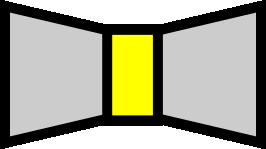
\includegraphics[scale=0.15]{auto-encoder-symbol.png}\hspace*{3pt}}}
\newcommand\squaref{\hspace*{-4pt}\raisebox{-2pt}{
		\tikz[scale=.3,thick]{
			\draw (0.3,0) to (0,0) to ++(-0.4,-1.1) to ++(-0.3,0);
			\draw (-0.6,-0.3) to ++(0.9,0);}%
}}
\newcommand\squareF{\hspace*{-1pt}\raisebox{-1pt}{
		\tikz[scale=.3,thick]{
			\draw (0.6,0) to (0,0) to ++(-0.2,-1);
			\draw (-0.1,-0.4) to ++(0.6,0);}%
}}
\newcommand*\circled[1]{\tikz[baseline=(char.base)]{
	\node[shape=circle,draw,inner sep=2pt] (char) {#1};}}

%% Import bib file for bibliography
\addbibresource{../AGI-book.bib}

\begin{document}

%% -------------------------------------------------
%% Thesis structure: In the order of
%% -------------------------------------------------
%% Titlepage  -> Authorization -> Signature ->
%% Acknowledgements ->
%% TOC -> List of Figures -> List of Tables ->
%% Abstract -> 
%% -------------------------------------------------
%% <Main body> -> 
%% -------------------------------------------------
%% References -> (Appendices)
%% -------------------------------------------------

\frontmatter
\maketitle 

\authorization
\signaturepage

\begin{acknowledgements}

Thank you, all the Evangelion.

\end{acknowledgements}


\tableofcontents
\listoffigures
\listoftables
% TODO: see \cmd{\newlistofalgorithms}
\newlistofalgorithms % This is to maintain the same appearance

%% Dedication and Preface are optional
%\begin{dedication}
  Dedicated to someone like you.
\end{dedication}

\begin{preface}

Some preface text.

\begin{flushright}
Author\\
2021. HK
\end{flushright}

\end{preface}

\begin{abstract}

Some text.

\end{abstract}


%% -------------------------------------------------
%% Main body
%% -------------------------------------------------
\mainmatter

\setcounter{chapter}{-1}
\chapter{Introduction}\label{chap:introduction}

\section{Background}

Lambek:
\begin{equation}
\begin{tikzcd}[row sep=1cm, column sep=0.6cm]
& \parbox{1.5cm}{\linespread{-0.5}\selectfont\centering type theory} \arrow[dl,dash] \arrow[dr,dash] & \\
\mbox{logic} \arrow[rr,dash] & {} & \parbox{1.5cm}{\linespread{-0.5}\selectfont\centering category theory}
\end{tikzcd}
\end{equation}

I am very curious to see if the two algebras below would coincide?
\begin{equation}
\begin{tikzcd}[row sep=1cm, column sep=0.6cm]
 & & \parbox{1.5cm}{\linespread{-0.5}\selectfont\centering type theory} \arrow[dl,dash] \arrow[dr,dash] & & & \\
\parbox{2cm}{\linespread{-0.5}\selectfont\centering algebraic logic} \arrow[rrrrr, dashed, dash, bend right] \arrow[r,dash] & \mbox{logic} \arrow[rr,dash] & {} & \parbox{1.5cm}{\linespread{-0.5}\selectfont\centering category theory} \arrow[r,dash] & \mbox{topos} \arrow[r,dash] & \parbox{2cm}{\linespread{-0.5}\selectfont\centering algebraic geometry}
\end{tikzcd}
\end{equation}

\section{Paul Halmos}

Every Boolean algebra $\mathbb{A}$ is isomorphic to the set of all continuous functions from $X$ into $\mathbb{O}$, where $X$ is the dual space of the algebra $\mathbb{A}$, and $\mathbb{O}$ is the Boolean algebra with 2 elements.  If there is a homomorphism $f$ between Boolean algebras $\mathbb{A} \rightarrow \mathbb{B}$ then there is a dual morphism $f^*$ between their dual spaces $Y \rightarrow X$:
\begin{equation}
\begin{tikzcd}[column sep=3cm, row sep=0.6cm]
\mathbb{A} \arrow[r,"f"] \arrow[d,shift left=2,phantom,"\cong"{anchor=south,rotate=90}] & \mathbb{B} \arrow[d,shift left=2,phantom,"\cong"{anchor=south,rotate=90}] \\
\overbracket{X} \arrow[d] & \overbracket{Y} \arrow[d] \arrow[l,"f^*"] \\
\underbracket{\mathbb{O}} & \underbracket{\mathbb{O}} 
\end{tikzcd}
\end{equation}

\section{The set-up}

The set of equations $F$ defines an algebraic set = \textbf{the world}:
\begin{equation}
F(x) = 0 .
\end{equation}
The objective of an intelligent agent is to learn $F$.

We have the function $f$ performing \textbf{prediction} of the immediate future:
\begin{equation}
\boxed{\mbox{current state}} \quad x_t \stackrel{f}{\mapsto} x_{t+1} \quad \boxed{\mbox{next state}} \;.
\end{equation}

In an infinitesimal sense, we can see $f$ as a \textbf{differential equation} describing the \textbf{world trajectory}:
\begin{equation}
\dot{x} = f(x) .
\end{equation}
So $F$ is the \textbf{solution} to this differential equation.

It seems that $F$ and $f$ are more or less equivalent ways to describe the world.

Logic can be turned into some form of algebra, and this algebra can be used to express either $F$ or $f$.  Perhaps both ways are feasible, or even mixing the two.

What does it mean to use logic to express $F$ or $f$?

The following table depicts the main correspondences relevant to our research:
\begin{equation}
\begin{tabular}{|c|c|c|}
	\hline
	\textbf{LOGIC} & \textbf{facts} & \textbf{rules} \\
		& \mbox{human(socrates)} & $\forall x. \mbox{human}(x) \rightarrow \mbox{mortal}(x)$ \\
	\hline
	\textbf{ALGEBRA} & \textbf{element} & \textbf{element} \\
		& $p \in \mathbb{A} $ & $(p \rightarrow q) \in \mathbb{A} $ \\
	\hline
	\textbf{WORLD} & \textbf{states} & \textbf{state transitions} \\
		& $x_t$ & $x_t \stackrel{f}{\mapsto} x_{t+1}$ \\
	\hline
\end{tabular}
\end{equation}
The relation between LOGIC and WORLD has been elucidated quite thoroughly in the AI literature.  Note that the state $x_t$ is made up of a set of facts (logic propositions).  A single step of logic inference results in a new conclusion $\delta x$ which is \textit{added} (as a set element) to the current state $x_t$ to form a new state $x_{t+1}$.  Here $t$ refers to ``mental time'' which does not necessarily coincide with real time.


% \chapter{Example chapter}\label{chap:sample}

\section{Background}\label{chap:exp:sec:background}

\subsection{Cross references}

You can use \lstinline|\cref{}| to automatically setup the cross reference name; instead, you can always use \lstinline|\ref{}| to customize the appearance of the cross reference.

Chapter \ref{chap:introduction} tells you to read the latest PDF documentation.

\cref{chap:conclusions} is a conclusion.

\subsection{Citation and bibliography}

Use \lstinline|biber| as \hologo{BibTeX} backend.

Cite a book\cite{LaTeX.Companion}, some papers\cite{KeshavACMSIGCOMMComput.Commun.Rev.2007, WhitesidesAdv.Mater.2004}, and a conference\cite{, Babu2020IEEE33rdInt.Conf.MicroElectroMech.Syst.MEMS2020}.

\subsubsection{Citation database}

Bibliography entries (database) are stored in \lstinline|mythesis.bib|. You can use Zotero (or similar software) to generate \lstinline|another.bib| file. You can add multiple database files by adding their filenames one-by-one in the following commands in \lstinline|mythesis.tex|:

\begin{lstlisting}[language=TeX]
\addbibresource{mythesis.bib}
\addbibresource{another.bib}
\end{lstlisting}

\subsubsection{Citation style}

As described in the sample page from ECE department, the style is set to \lstinline|ieee| by default. You can modify the style in the \lstinline|hkustthesis.cls| file as you wish.

\section{Math}

\subsection{Symbols}

\begin{itemize}
  \item Calligraphic letters: $\mathcal{A}$
  \item Mathbb letters: $\mathbb{A}$
  \item Mathfrak letters: $\mathfrak{A}$
  \item Math Sans serif letters: $\mathsf{A}$
  \item Math bold letters: $\mathbf{A}$
  \item Math bold upright Greek letters: $\mathbf{\alpha}$ (Not displaying! Use the following one.)
  \item Math bold upright Greek letters: $\symbfup{\alpha}$
\item Math bold italic Greek letters\footnote{Avoid using \lstinline|bm| package as it conflicts with \lstinline|unicode-math| and it is outdated for \hologo{XeLaTeX}. You can alias some math commands by \lstinline|\\newcommand| or \lstinline|\\renewcommand| anyway.}: $\bm{\alpha}$
  \item Math bold italic Greek letters in upper case: $\mathbi{A}$
\end{itemize}

\subsection{Equations}

\begin{equation}
  E^2 = m^2 + p^2\label{eq:mass-energy}
\end{equation}

\cref{eq:mass-energy} or Equation (\ref{eq:mass-energy}) gives the mass-energy relationship.

\subsection{Theorem}

\begin{definition}
  LCL is orange juice.
\end{definition}

\begin{proof}
  They are both orange.
\end{proof}

\begin{algorithm}[htbp]
  \caption{Temp}
  \begin{algorithmic}[1]
    \STATE Temp
  \end{algorithmic}
\end{algorithm}

Available theorem environments are listed below:

algorithm, assumption, axiom, conclusion, condition, corollary, definition, example, lemma, proof, property, proposition, remark, theorem.

\section{Figure}
An example image is shown in \cref{fig:tikz example} or Figure (\ref{fig:tikz example}).

\begin{figure}[H]
  \centering
  \begin{tikzpicture}
    \draw (0,0) -- (1, 0) -- (1, 1) -- cycle;
  \end{tikzpicture}
  \caption{An example tikz picture with a short caption.}
  \label{fig:tikz example short}
\end{figure}

\begin{figure}[H]
  \centering
  \begin{tikzpicture}
    \draw (0,0) -- (1, 0) -- (1, 1) -- cycle;
  \end{tikzpicture}
  \caption{An example tikz picture with breakline and\\ a very very very very very very very very very very very very very very very very very very very very very very very very very very very very very very very long caption.}
  \label{fig:tikz example}
\end{figure}

\section{Table}

An example table is shown in \cref{tab:environment} or Table (\ref{tab:environment}).

\begin{table}[H]
  \centering
  \caption{A table with a short caption.}
  \label{tab:table_short}
  \begin{tabular}{lll}
    \toprule
    OS           & TeX environment                & Test                                \\
    \midrule
    Overleaf     & \hologo{TeX}\,Live 2021$\sim$4 & Pass                                \\
    Windows 10   & \hologo{TeX}\,Live 2020        & \color{red}{\verb|ltxhook| problem} \\
    Ubuntu 20.04 & \hologo{TeX}\,Live 2021        & Pass                                \\
    \bottomrule
  \end{tabular}
\end{table}

\begin{table}[H]
  \centering
  \caption{Test result on different platforms with breakline and\\ a very very very very very very very very very very very very very very very very very very very very very very very very very very very very very very very long caption.}
  \label{tab:environment}
  \begin{tabular}{lll}
    \toprule
    OS                   & TeX environment                & Test                                \\
    \midrule
    Overleaf             & \hologo{TeX}\,Live 2021$\sim$4 & Pass                                \\
    Arch Linux (2024.10) & \hologo{TeX}\,Live             & Pass                                \\
    Windows 10/11        & \hologo{TeX}\,Live 2021        & Pass                                \\
    macOS 10.15          & \hologo{TeX}\,Live 2021        & Pass                                \\
    Windows 10           & \hologo{TeX}\,Live 2020        & \color{red}{\verb|ltxhook| problem} \\
    Ubuntu 20.04         & \hologo{TeX}\,Live 2021        & Pass                                \\
    Termux               & \hologo{TeX}\,Live 2021        & Pass                                \\
    Windows 11           & \hologo{MiKTeX} 4.9            & Pass                                \\
    Windows 10           & \hologo{MiKTeX} 4.4            & Pass                                \\
    \bottomrule
  \end{tabular}
\end{table}

\section{Code}

\subsection{Inline code}
Use \lstinline$\lstinline|<code>|$ to print code snippets. The \lstinline$||$ marks delimit
the code and can be replaced by any character not in the code;
\eg \lstinline|\lstinline$<code>$| gives the same result.

\subsection{Code environment}
The code to draw the \cref{fig:tikz example} is listed below:
\begin{lstlisting}[caption={\hologo{LaTeX} code for inserting a figure}]
\begin{figure}[htb]
  \begin{tikzpicture}
    \draw (0,0) -- (1, 0) -- (1, 1) -- cycle;
  \end{tikzpicture}
  \caption{An example picture with long caption: \blindtext\\\blindtext}
  \label{fig:tikz example} % this is a comment
\end{figure}
\end{lstlisting}

\chapter{Background: The mind as a dynamical system}\label{chap:background1}

\section{The set-up}

The set of equations $F$ defines an algebraic set = \textbf{the world}:
\begin{equation}
F(x) = 0 .
\end{equation}
The objective of an intelligent agent is to learn $F$.

We have the function $f$ performing \textbf{prediction} of the immediate future:
\begin{equation}
\boxed{\mbox{current state}} \quad x_t \stackrel{f}{\mapsto} x_{t+1} \quad \boxed{\mbox{next state}} \;.
\end{equation}

In an infinitesimal sense, we can see $f$ as a \textbf{differential equation} describing the \textbf{world trajectory}:
\begin{equation}
\dot{x} = f(x) .
\end{equation}
So $F$ is the \textbf{solution} to this differential equation.

It seems that $F$ and $f$ are more or less equivalent ways to describe the world.

Logic can be turned into some form of algebra, and this algebra can be used to express either $F$ or $f$.  Perhaps both ways are feasible, or even mixing the two.

What does it mean to use logic to express $F$ or $f$?

Go back to a physics example, the parabolic trajectory of a canon ball:
\begin{equation}
\vcenter{\hbox{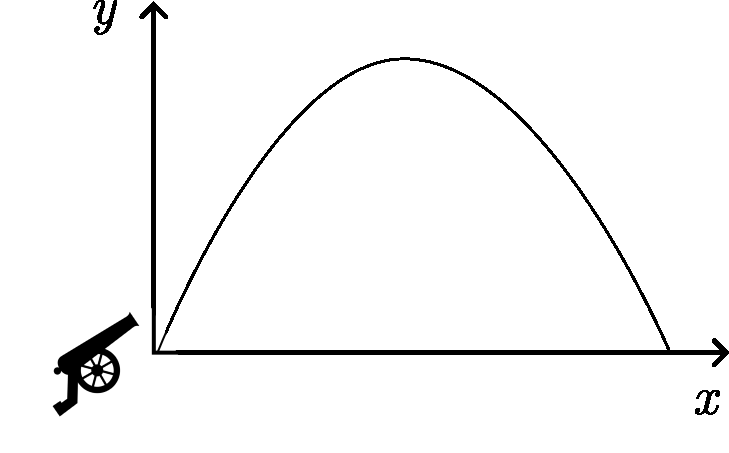
\includegraphics[scale=0.7]{canonball-parabola.png}}}
\end{equation}
The parabola is given by the quadratic equation from high school:
\begin{equation}
F(x) = 0 \qquad F(x) = ax^2 + bx + c
\end{equation}
but the trajectory can also be described by the physics equation parameterized by time $t$:
\begin{equation}
\dot{\mathbf{x}} = f(\mathbf{x}) = (v_x, v_y) = (v^0_x , -gt + v^0_y) .
\end{equation}
This parametric form is not unique.  For example, another way is for the point $\mathbf{x}$ to move with uniform speed along the trajectory.

Note that the trajectory above is qualitatively the same as a ``thought trajectory'' in cognitive space.  One intuitive way to visualize cognitive trajectories is via the example of a chess game tree (where the opponent's move is regarded as how the ``world'' reacts to the agent's actions):
\begin{equation}
\vcenter{\hbox{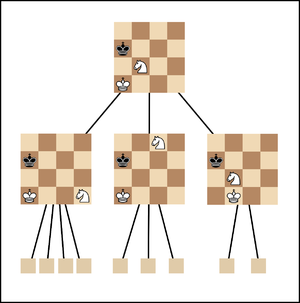
\includegraphics[scale=0.7]{chess-game-tree.png}}}
\end{equation}

$f(x)$ is the functional form we want, as it contains information about the ``interestingness'' of deduced conclusions.

Are our equations in Table \ref{table:formulas} describing $F$ or $f$?  

An intuitive idea:  state = facts = grounded equations, rules = quantified equations.  So the equations are modeling $f$.  This exposed a problem of classical AI that I have not paid too much attention to:  the selection of interesting conclusions.  It's hard to \textbf{enumerate conclusions}, let alone to rate their interestingness.

		% Dynamical system
\chapter{Background: Categorical logic}\label{chap:background2}

Lambek posited this ``trinity'':
\begin{equation}
\begin{tikzcd}[row sep=1cm, column sep=1cm]
& \parbox{1.5cm}{\linespread{-0.5}\selectfont\centering type theory} \arrow[dl,dash,"Curry-","Howard"',sloped] \arrow[dr,dash,"\text{obvious}",sloped] & \\
\mbox{logic} \arrow[rr,shift left=2pt,harpoon,"\text{classifying topos}"]  & {} & \parbox{1.5cm}{\linespread{-0.5}\selectfont\centering category theory}
\arrow[ll, shift left=2pt, harpoon, "\text{internal language}"]
\end{tikzcd}
\end{equation}
where the double arrows at the base can be understood thusly:


I extended some nodes to better see their relations:
\begin{equation}
\begin{tikzcd}[row sep=1cm, column sep=0.6cm]
& & \parbox{1.5cm}{\linespread{-0.5}\selectfont\centering type theory} \arrow[dl,dash] \arrow[dr,dash] & & & \\
\parbox{2cm}{\linespread{-0.5}\selectfont\centering algebraic logic} \arrow[rrrrr, dashed, dash, bend right,"?"] \arrow[r,dash] & \mbox{logic} \arrow[rr,dash] & {} & \parbox{1.5cm}{\linespread{-0.5}\selectfont\centering category theory} \arrow[r,dash] & \mbox{topos} \arrow[r,dash] & \parbox{2cm}{\linespread{-0.5}\selectfont\centering algebraic geometry}
\end{tikzcd}
\end{equation}
I am curious if the two algebras on the left and right are identical?

\section{Topos and internal language}

		% Categorical logic
\chapter{Background: Algebraic logic}\label{chap:background3}

\section{Paul Halmos' algebraic logic}

The essence of Halmos' approach to algebraic logic may be explained by this diagram:
\begin{equation}
\vcenter{\hbox{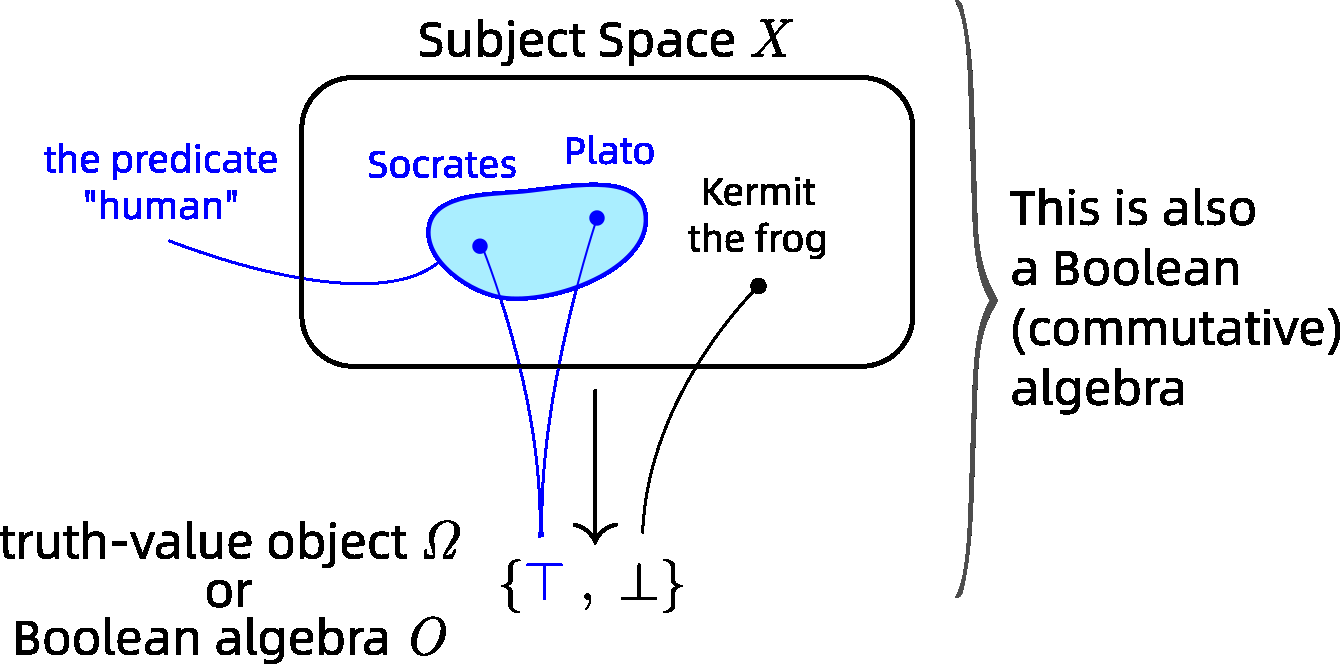
\includegraphics[scale=0.6]{Halmos-nutshell.png}}}
\end{equation}
I coined the term ``Subject Space'' to refer to the space of \textbf{subjects} referred to by predicates.  For example the predicate $\logic{mortal}(\_)$ applies to subjects such as $\logic{Socrates}$ and $\logic{Plato}$ but does not apply to the subject $\logic{Zeus}$.

We all know that propositional logic is isomorphic to the Boolean algebra of sets (Stone's duality theorem).  This is the basis of treating logic as algebra.  But the most tricky point of algebraizing a logic is the treatment of \textbf{predicates}.  Halmos observed that one can form \textbf{propositional functions} from a Subject Space $X$ to a Boolean algebra, and the resulting set of functions would still be a Boolean algebra.  In the above diagram we can see a function mapping subjects to the set $\{ \top, \bot \}$ which is the minimal Boolean algebra $O$, containing only 2 elements, true and false.

The target domain can be a more complex Boolean algebra, as in $X \rightarrow A$.  For example, if Achilles was Zeus's son, he would also be immortal.  So in the proposition space $A$, there would be an implication arrow $\logic{immortal}(\logic{Zeus}) \rightarrow \logic{immortal}(\logic{Achilles})$.  Note that the space $A$ contains points which are just propositions, we cannot access their internal structure.  Anyway, I find that $O = \{ \top, \bot \}$ suffices for our purposes, and we don't need the richer structure of $A$.

More technically, we have the following duality.  Every Boolean algebra $\mathbb{A}$ is isomorphic to the set of all continuous functions from $X$ into $\mathbb{O}$, where $X$ is the dual space of the algebra $\mathbb{A}$, and $\mathbb{O}$ is the Boolean algebra with 2 elements.  If there is a homomorphism $f$ between Boolean algebras $\mathbb{A} \rightarrow \mathbb{B}$ then there is a dual morphism $f^*$ between their dual spaces $Y \rightarrow X$:
\begin{equation}
\begin{tikzcd}[column sep=3cm, row sep=0.6cm]
\mathbb{A} \arrow[r,"f"] \arrow[d,shift left=2,phantom,"\cong"{anchor=south,rotate=90}] & \mathbb{B} \arrow[d,shift left=2,phantom,"\cong"{anchor=south,rotate=90}] \\
\overbracket{X} \arrow[d] & \overbracket{Y} \arrow[d] \arrow[l,"f^*"] \\
\underbracket{\mathbb{O}} & \underbracket{\mathbb{O}} 
\end{tikzcd}
\end{equation}

\section{An ``algebraic geometry'' idea from Yuri Manin and Russians}

Please refer to the next 4 pages excerpted from the book \textit{Geometry I: Basic Ideas and Concepts of Differential Geometry}, by some Russian authors from 1991 \cite{Alekseevskij1991}.  They attributed the idea to Yuri Manin.

Halmos' algebraization is quite straightforward:  predicates are simply functions from Subject Space to truth values.  Yuri Manin's approach brings \textbf{algebraic geometry} into the picture:  Suppose $\mathbb{A}$ is a Boolean algebra.  An element $P \in \mathbb{A}$ can be understood as an $\mathbb{F}_2$-valued function (ie, taking truth values 0 or 1) on the set $\Spec \mathbb{A}$.  The subset $M_P \subset \Spec \mathbb{A}$ consists of those objects for which the statement $P$ is true.  In our terminology, $P$ is a predicate, $M_P$ is the subset for which $P$ is true, $\Spec \mathbb{A} = X =$ Subject Space, and ``points'' in Subject Space are maximal (or prime) ideals of the algebra $\mathbb{A}$.

Any ring can be considered a ring of functions over a space $X$.  The ``points'' of $X$ correspond to homomorphisms from the ring into certain fields.  We can view them as maximal (or prime) ideals of the ring.

% The structure sheaf (a commutative ring) sits above a site which is an algebraic variety endowed with a topology.  

% My understanding is that \textbf{Boolean algebra} and \textbf{Boolean rings} are essentially synonymous.  Both can be regarded as a form of propositional logic.

\textbf{Stone duality} provides the link between Boolean algebra and the algebra of sets (of a topological space).  Halmos' algebraization provides a simple way to extend this to predicate logic.  Manin's idea coincides with Halmos', but it offers a deeper, algebraic-geometric perspective.

\begin{figure}
\tcbincludegraphics[hbox,colframe=blue,boxrule=1pt,arc=0pt,outer arc=0pt,graphics options={scale=0.5}]{Geometry-I-a.png}
\end{figure}

\begin{figure}
\tcbincludegraphics[hbox,colframe=blue,boxrule=1pt,arc=0pt,outer arc=0pt,graphics options={scale=0.5}]{Geometry-I-b.png}
\end{figure}

\begin{figure}
\tcbincludegraphics[hbox,colframe=blue,boxrule=1pt,arc=0pt,outer arc=0pt,graphics options={scale=0.5}]{Geometry-I-c.png}
\end{figure}

\begin{figure}
\tcbincludegraphics[hbox,colframe=blue,boxrule=1pt,arc=0pt,outer arc=0pt,graphics options={scale=0.5}]{Geometry-I-d.png}
\end{figure}

\section{``Term rewriting and all that''}

From the book of that title \cite{Baader1998}.  In Chapter 8, \textit{Gr\"{o}bner bases and Buchberger's Algorithm}, a correspondence is made between Huet's \textbf{higher-order unification} algorithm and Buchberger's algorithm for finding Gr\"{o}bner bases.

An interesting question is whether this correspondence fits into our framework of algebraic logic.  I need more time to determine this...

\begin{equation}
\vcenter{\hbox{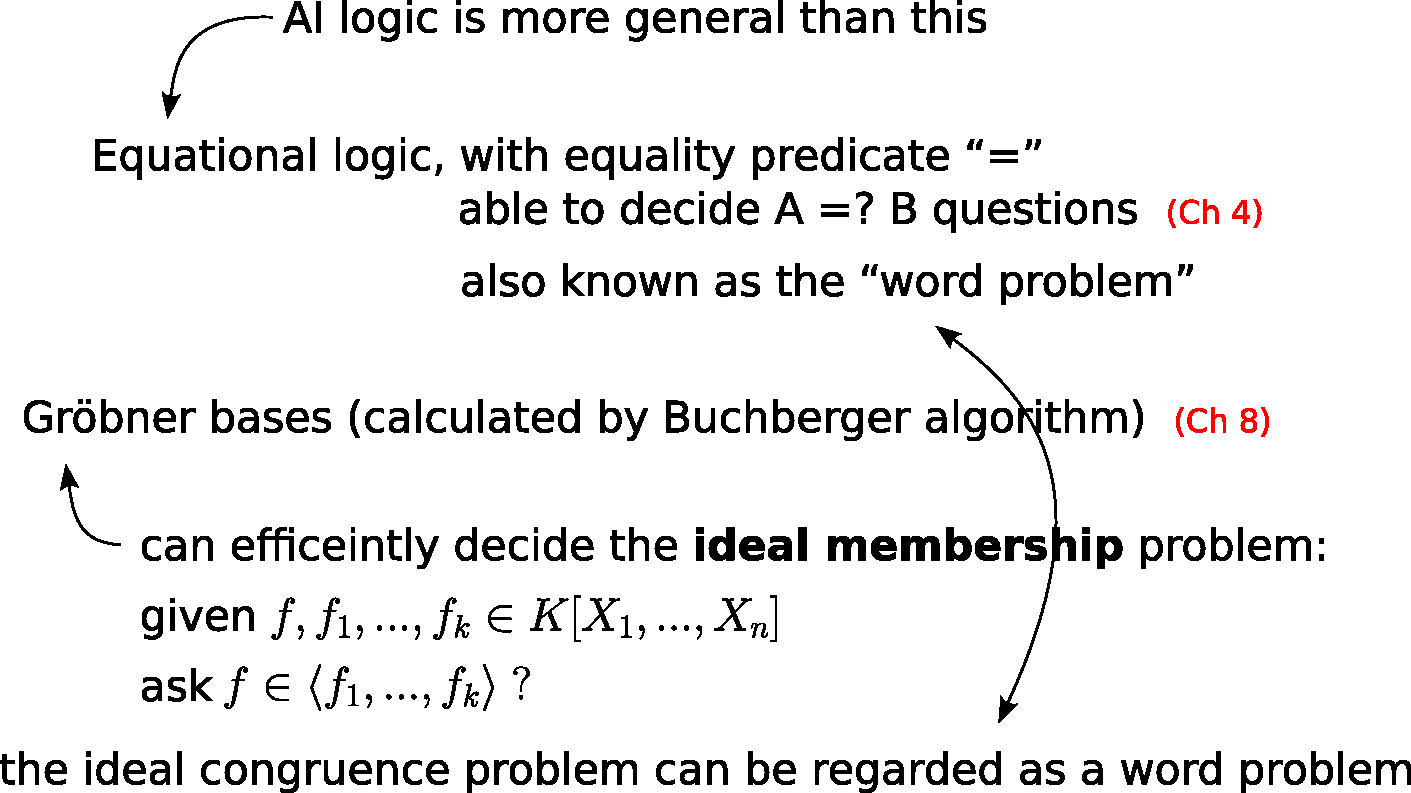
\includegraphics[scale=0.7]{term-rewriting-and-all-that.png}}}
\end{equation}

\begin{itemize}
	\item What is the \textbf{word problem}? \\
	is defined for an equational theory $E$. \\
	is the problem of deciding whether $s = t$
	
	\item why is Gr\"{o}bner basis equivalent to the word problem? \\
	to ask ideal congruence $f =? g$ means $f - g \in? J$ \\
	which is ideal membership problem \\
	a polynomial can be regarded as a rewrite rule \\
	because $f = 0$, we can take the ``largest monomial'' in $f$ as the LHS, and the rest of $f$ as RHS. \\
	In other words:  ideal = set of rules \\
	We ask if a polynomial can be rewritten by the set of rules to another form.  \\
	This is similar to logic deduction.
	
	\item Here an important question is: polynomial reduction seems unable to handle \textbf{logic variables}, it seems only capable of \textbf{simple symbolic rewriting}.
	
	\item logic is equivalent to what form of polynomials? \\
	taking the cue that Huet's higher-order unification = Buchberger algorithm, ...
\end{itemize}

This is now a big topic, e.g. the book \textit{Algebraic Operads -- An Algorithmic Companion} \cite{Bremner2016}.  Writing the \textbf{normal forms} of elements of an algebra is accomplished by the \textbf{diamond lemma}.  One approach is by eliminating leading terms of the ideal generated by given polynomials.  A Gr\"{o}bner basis is one for the quotient of a polynomial algebra by an ideal.  

\section{How to study symmetries in deep learning?}

In the following, we will use this sentence as example:
\begin{equation}
	\mbox{\textit{The quick brown fox jumps over the lazy dog}}
\end{equation}
which is a sequence of length $n = 9$.

Matrix formula for Self-Attention:
\begin{align}
	Q &= W^Q X \nonumber \\
	K &= W^K X \nonumber \\
	V &= W^V X \nonumber \\
	\boxed{\mbox{output}} \quad  Z &= \mathrm{softmax} \left( \frac{ Q K^\top }{\sqrt{d_k}} \right) V
	\label{eqn:self-attention}
\end{align}
Take the convention that $X$ consists of ``word vectors'' as \textbf{row} vectors, stacked up to form a matrix of height $n$ which is the sequence length.  The equivariant symmetry says that if we swap any two row vectors in $X$, then the output $Z$ would also have the same rows swapped.  Is this symmetry easy to spot from equation \ref{eqn:self-attention}?  (Note: softmax does not change the structure of its matrix argument, so structurally the output matrix is just $QK^\top V$.)  Perhaps if the reader is very good at linear algebra, but I could not see it.

Figure (\ref{fig:self-attention}) makes it easier to see the matrices' dimensions, but the symmetry is still not apparent.
\begin{figure}
\begin{equation}
\vcenter{\hbox{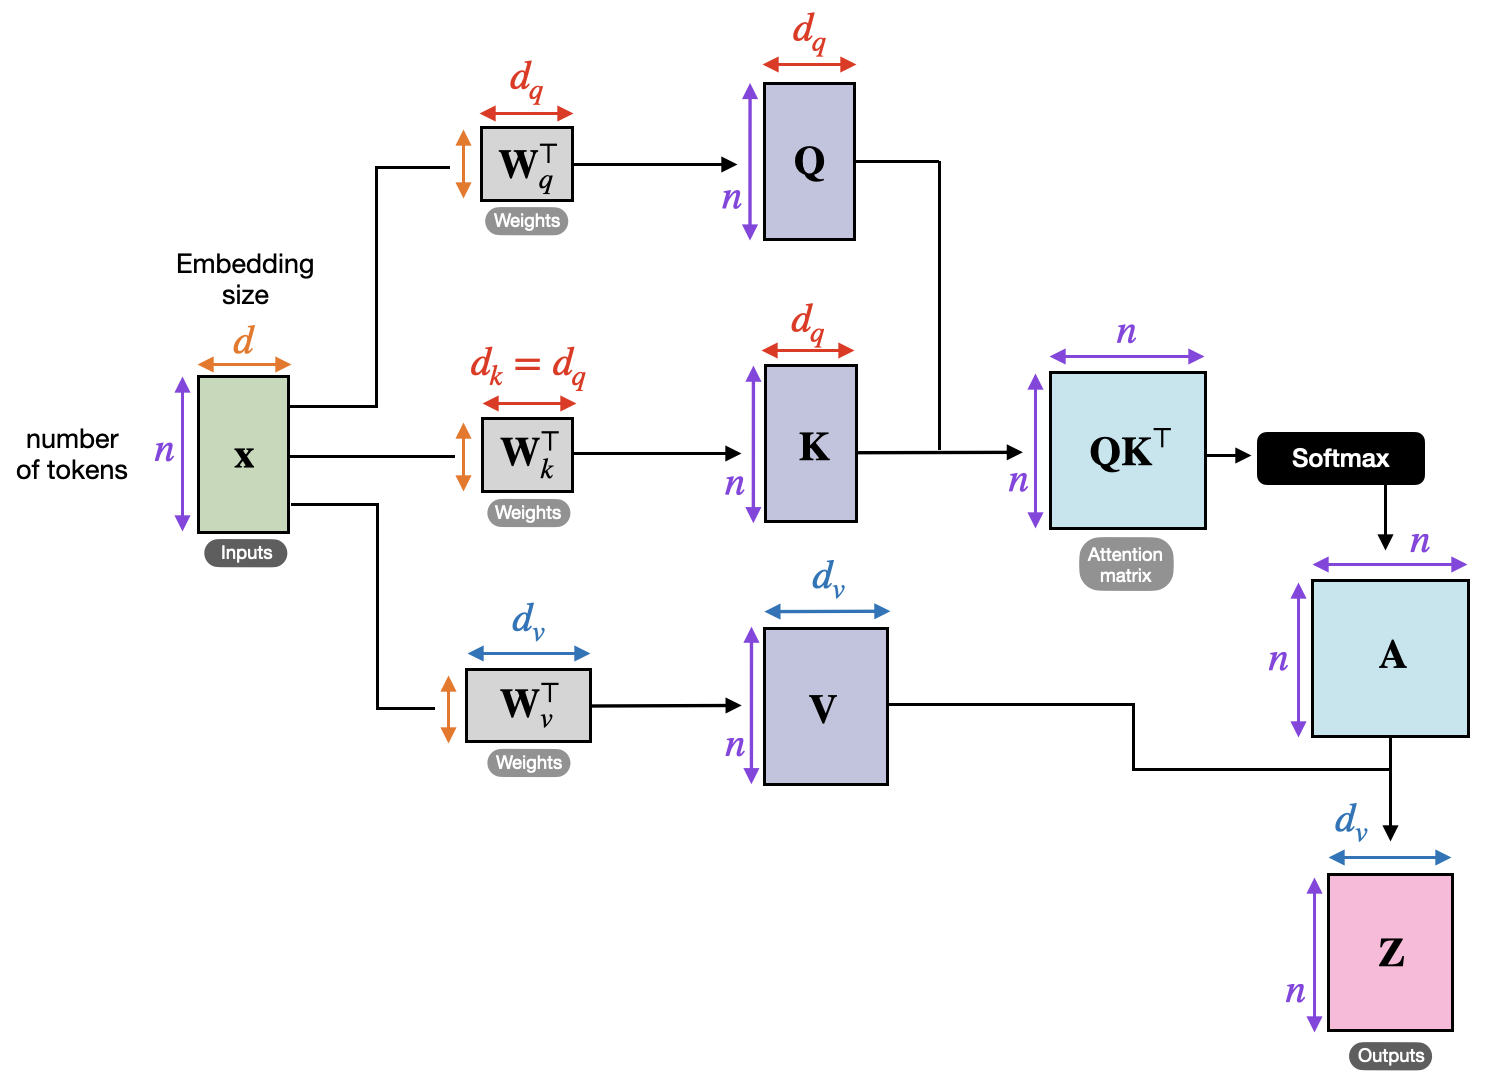
\includegraphics[scale=0.5]{self-Attention.png}}}
\label{fig:self-attention}
\end{equation}
\end{figure}

The way I ``see'' the symmetry can be described verbally as follows:  Imagine \textit{Fox} and \textit{Dog} swapped positions at the input.  The table-lookup operations $W^Q, W^K$ and $W^V$ do not change the rows structure.  When \textit{Fox} is the \textbf{pivot} of its rule, it is matched against Key Key ... Key (which are the same keys as would be matched against \textit{Dog}).  The result for \textit{Fox}'s matching would be a row vector of length $n$, same as for \textit{Dog}.  Since there are $n$ words in the sequence, and each matching involves $n$ keys, the results make up a $n \times n$ matrix, which we call the \textbf{Attention matrix} (after applying softmax, but softmax does not change the structure of the matrix).  In the final matrix multiplication, $[d_V \times n] \times [n \times n] \rightarrow [d_V \times n]$, where one common dimension $n$ on each side has been ``destroyed'' by \textbf{contraction} (dot product).  Another way to say this, not using dot product, is that we have $n$ Value vectors, each Value vector is weighted by one row of the Attention matrix and then added together, resulting in a new Value vector.  This is repeated $n$ times to give $[d_V, n]$.

The following diagrams try to show the equivariance property of Self-Attention:
\begin{figure}
	\begin{equation}
	\hspace{-1.5cm}\vcenter{\hbox{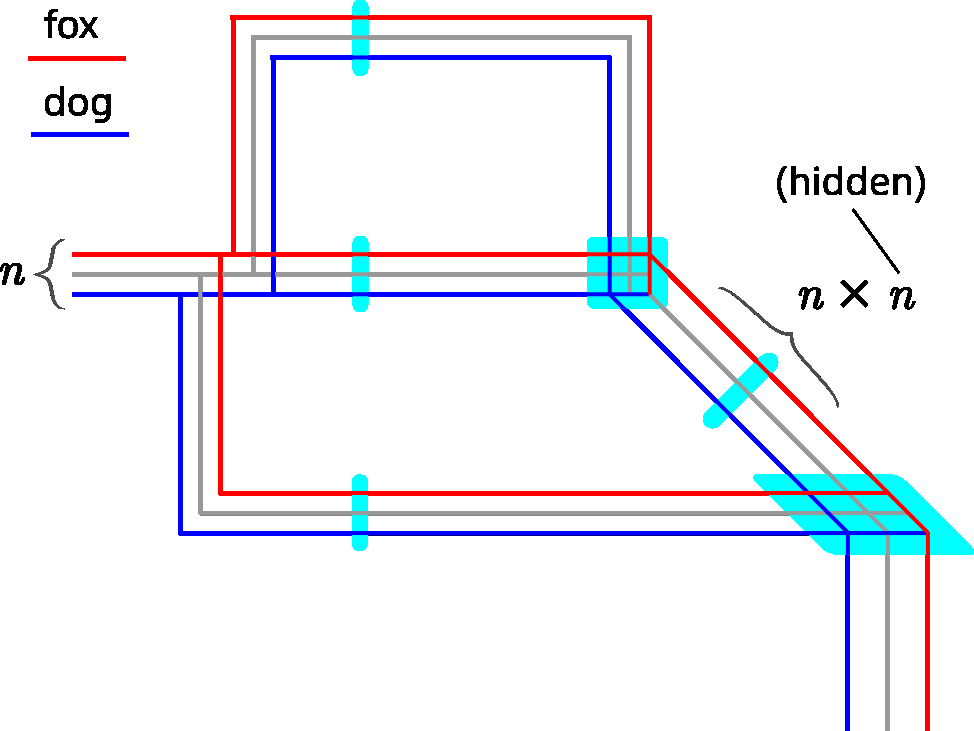
\includegraphics[scale=0.6]{self-attention-string-diagram-2.png}}}
	\qquad
	\vcenter{\hbox{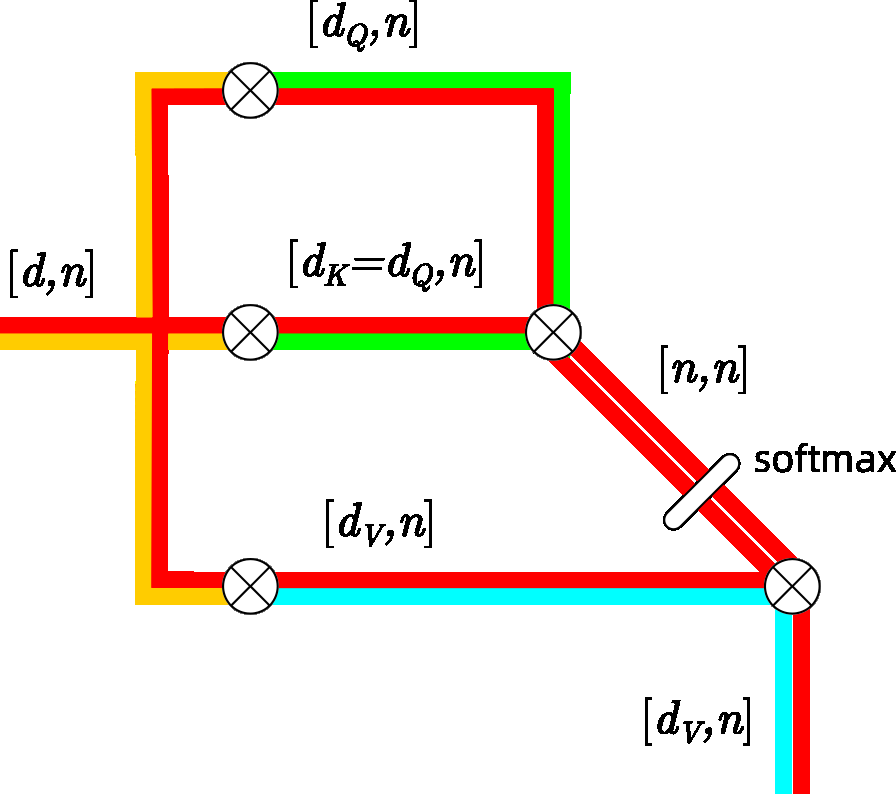
\includegraphics[scale=0.6]{self-attention-string-diagram-3.png}}}
	\label{fig:self-attention-2-and-3}
	\end{equation}
\end{figure}
The diagram on the left shows a single dimension which is $n$.  The diagram on the right shows all dimensions in different colors.

The simplest example of an equivariance:
\begin{equation}
% method to draw a sigmoid-shape curve:
% \draw (0,0) .. controls (0,4) and (4,0) .. (4,4);
% the controls acts like "magnets"
\begin{tikzpicture}[every path/.style={thick}]
\node[] (x0) at (-3, 0) {};
\node[] (x1) at (-3, 0.5) {};
\node[] (1i) at (-2.7, 0.5) {};
\node[] (1j) at (-1.7, 0.5) {};
\node[] (x2) at (-3, 1) {};
\node[] (x3) at (-3, 1.5) {};
\node[] (3i) at (-2.7, 1.5) {};
\node[] (3j) at (-1.7, 1.5) {};
\node[] (x4) at (-3, 2) {};
\node[] (x5) at (-3, 2.5) {};
\node[] (y0) at (3, 0) {};
\node[] (y1) at (3, 0.5) {};
\node[] (y2) at (3, 1) {};
\node[] (y3) at (3, 1.5) {};
\node[] (y4) at (3, 2) {};
\node[] (y5) at (3, 2.5) {};
\draw (x0) to (y0);
\draw[red] (x1) to (1i.center);
    \draw[red] (1i.center) to[out=0,in=-180] (3j.center);
    \draw[red] (3j.center) to (y3);
\draw (x2) to (y2);
\draw[blue] (x3) to (3i.center);
    \draw[blue] (3i.center) to[out=0,in=-180] (1j.center);
    \draw[blue] (1j.center) to (y1);
\draw (x4) to (y4);
\draw (x5) to (y5);
\end{tikzpicture}
\qquad \raisebox{3em}{=} \qquad
\begin{tikzpicture}[every path/.style={thick}]
\node[] (x0) at (-3, 0) {};
\node[] (x1) at (-3, 0.5) {};
\node[] (1i) at (1.7, 0.5) {};
\node[] (1j) at (2.7, 0.5) {};
\node[] (x2) at (-3, 1) {};
\node[] (x3) at (-3, 1.5) {};
\node[] (3i) at (1.7, 1.5) {};
\node[] (3j) at (2.7, 1.5) {};
\node[] (x4) at (-3, 2) {};
\node[] (x5) at (-3, 2.5) {};
\node[] (y0) at (3, 0) {};
\node[] (y1) at (3, 0.5) {};
\node[] (y2) at (3, 1) {};
\node[] (y3) at (3, 1.5) {};
\node[] (y4) at (3, 2) {};
\node[] (y5) at (3, 2.5) {};
\draw (x0) to (y0);
\draw[red] (x1) to (1i.center);
	\draw[red] (1i.center) to[out=0,in=-180] (3j.center);
	\draw[red] (3j.center) to (y3);
\draw (x2) to (y2);
\draw[blue] (x3) to (3i.center);
	\draw[blue] (3i.center) to[out=0,in=-180] (1j.center);
	\draw[blue] (1j.center) to (y1);
\draw (x4) to (y4);
\draw (x5) to (y5);
\end{tikzpicture}
\end{equation}

Illustration of a function $\vec{f}$ with \textbf{equivariance} property:
\begin{equation}
% method to draw a sigmoid-shape curve:
% \draw (0,0) .. controls (0,4) and (4,0) .. (4,4);
% the controls acts like "magnets"
\begin{tikzpicture}[every path/.style={thick}]
\node[red,above] (x0) at (0, 3) {${\scriptstyle f_1(\vec{v})}$};
\node[blue,above] (x1) at (1, 3) {${\scriptstyle f_2(\vec{v})}$};
\node[above] (x2) at (2, 3) {${\scriptstyle f_3(\vec{v})}$};
\node[] (z0) at (0, 1.5) {};
\node[] (z1) at (1, 1.5) {};
\node[] (z2) at (2, 1.5) {};
\node[red,below] (v0) at (0, 0) {$v_1$};
\node[blue,below] (v1) at (1, 0) {$v_2$};
\node[below] (v2) at (2, 0) {$v_3$};
\draw[red] (x0) to (z0.center);
\draw[blue] (x1) to (z1.center);
\draw (x2) to (z2.center);
\draw[red] (z0.center) to (v0);
\draw[blue] (z1.center) to (v1);
\draw (z2.center) to (v2);
\node[inner xsep=40pt,draw,in front of path,fill=white] (f) at (1,1.8) {$\vec{f}$};
\end{tikzpicture}
\qquad \raisebox{5em}{;} \qquad
\begin{tikzpicture}[every path/.style={thick}]
\node[blue,above] (x0) at (0, 3) {${\scriptstyle f_2(\vec{v})}$};
\node[red,above] (x1) at (1, 3) {${\scriptstyle f_1(\vec{v})}$};
\node[above] (x2) at (2, 3) {${\scriptstyle f_3(\vec{v})}$};
\node[] (z0) at (0, 1.5) {};
\node[] (z1) at (1, 1.5) {};
\node[] (z2) at (2, 1.5) {};
\node[red,below] (v0) at (0, 0) {$v_1$};
\node[blue,below] (v1) at (1, 0) {$v_2$};
\node[below] (v2) at (2, 0) {$v_3$};
\draw[blue] (x0) to (z0.center);
\draw[red] (x1) to (z1.center);
\draw (x2) to (z2.center);
\draw[blue] (z0.center) .. controls (0,0.3) and (1,1.2) .. (v1);
\draw[red] (z1.center) .. controls (1,0.3) and (0,1.2) .. (v0);
\draw (z2.center) to (v2);
\node[inner xsep=40pt,draw,in front of path,fill=white] (f) at (1,1.8) {$\vec{f}$};
\end{tikzpicture}
\qquad \raisebox{5em}{=} \qquad
\begin{tikzpicture}[every path/.style={thick}]
\node[blue,above] (x0) at (0, 3) {${\scriptstyle f_2(\vec{v})}$};
\node[red,above] (x1) at (1, 3) {${\scriptstyle f_1(\vec{v})}$};
\node[above] (x2) at (2, 3) {${\scriptstyle f_3(\vec{v})}$};
\node[] (z0) at (0, 1.5) {};
\node[] (z1) at (1, 1.5) {};
\node[] (z2) at (2, 1.5) {};
\node[red,below] (v0) at (0, 0) {$v_1$};
\node[blue,below] (v1) at (1, 0) {$v_2$};
\node[below] (v2) at (2, 0) {$v_3$};
\draw[blue] (x0) .. controls (0,1.8) and (1,2.7) .. (z1.center);
\draw[red] (x1) .. controls (1,1.8) and (0,2.7) .. (z0.center);
\draw (x2) to (z2.center);
\draw[red] (z0.center) to (v0);
\draw[blue] (z1.center) to (v1);
\draw (z2.center) to (v2);
\node[inner xsep=40pt,draw,in front of path,fill=white] (f) at (1,1) {$\vec{f}$};
\end{tikzpicture}
\end{equation}

If $\vec{f}$ is \textbf{invariant}, the diagram would be:
\begin{equation}
\begin{tikzpicture}[every path/.style={thick}]
\node[above] (x0) at (0, 3) {${\scriptstyle f_1(\vec{v})}$};
\node[above] (x1) at (1, 3) {${\scriptstyle f_2(\vec{v})}$};
\node[above] (x2) at (2, 3) {${\scriptstyle f_3(\vec{v})}$};
\node[] (z0) at (0, 1.5) {};
\node[] (z1) at (1, 1.5) {};
\node[] (z2) at (2, 1.5) {};
\node[red,below] (v0) at (0, 0) {$v_1$};
\node[blue,below] (v1) at (1, 0) {$v_2$};
\node[below] (v2) at (2, 0) {$v_3$};
\draw[red] (x0) to (z0.center);
\draw[blue] (x1) to (z1.center);
\draw (x2) to (z2.center);
\draw[blue] (z0.center) .. controls (0,0.3) and (1,1.2) .. (v1);
\draw[red] (z1.center) .. controls (1,0.3) and (0,1.2) .. (v0);
\draw (z2.center) to (v2);
\node[inner xsep=40pt,draw,in front of path,fill=white] (f) at (1,1.8) {$\vec{f}$};
\end{tikzpicture}
\qquad \raisebox{5em}{=} \qquad
\begin{tikzpicture}[every path/.style={thick}]
\node[above] (x0) at (0, 3) {${\scriptstyle f_1(\vec{v})}$};
\node[above] (x1) at (1, 3) {${\scriptstyle f_2(\vec{v})}$};
\node[above] (x2) at (2, 3) {${\scriptstyle f_3(\vec{v})}$};
\node[] (z0) at (0, 1.5) {};
\node[] (z1) at (1, 1.5) {};
\node[] (z2) at (2, 1.5) {};
\node[red,below] (v0) at (0, 0) {$v_1$};
\node[blue,below] (v1) at (1, 0) {$v_2$};
\node[below] (v2) at (2, 0) {$v_3$};
\draw[red] (x0) to (z0.center);
\draw[blue] (x1) to (z1.center);
\draw (x2) to (z2.center);
\draw[red] (z0.center) to (v0);
\draw[blue] (z1.center) to (v1);
\draw (z2.center) to (v2);
\node[inner xsep=40pt,draw,in front of path,fill=white] (f) at (1,1.8) {$\vec{f}$};
\end{tikzpicture}
\end{equation}

Practical TO-DO:
\begin{itemize}
	\item implement neural second-order or higher-order logic
	\item enable the creation of random constants (is it useful?)
	\item clarify the role of predicates in HOL, esp its geometric interpretation
\end{itemize}

% 其实想问问就是: 现时理论还能为我们做什么?
% 逻辑 含有「更强」的对称性,但这确切地是什么意思?
% 问题是,暂时我们不太懂得如何量度任意的对称性
% 对称性即「约束」,但此又引申到 参数空间大小的问题
% 如果 参数空间的大小不变,对称性仍可以有强弱之分
% 而以上的观测是严格成立的
% 所以可以说,对称性就是: 在参数空间一样大的情况下,
% 为什么我们说 Attention 比 fully connected 有更强对称性?
% 对称性似乎是相对于 input-output 而言的

The question now is:  what can abstract theory do for us?  We wish to be able to ``compare'' the symmetries possessed by systems.  When doing so, it is important to \textbf{restrict} the number of parameters for all systems in consideration.  This restriction comes from limited computing resource, without which it is meaningless to compare architectures.  After we fixed the number of parameters, two systems, such as fully-connected vs Transformer, could still be different as one possesses equivariant symmetry while the other does not.  This difference in symmetry is what I argue to be crucial to acceleration.

In its most general form an AGI system is defined by the transition function $X_{t+1} = \squareF(X_t)$.  A symmetry can be defined as any group $G$ such that $\squareF$ is invariant or equivariant under its action on the input $X$.  For example, $\squareF(\sigma X) = \sigma \squareF(X), \forall \sigma \in G$.  More generally, any constraint on $\squareF$ could result in acceleration, such as an equation satisfied by $\squareF$.

What is the relation between equivariance of Attention and symmetric NNs of Kolmogorov-Arnold type?

Rewrite neural string diagrams, how?
		% Algebraic logic
\chapter{Design of algorithm}\label{chap:algorithm}

The following table depicts the main correspondences relevant to our research:
\begin{equation}
\begin{tabular}{|c|c|c|}
\hline
\textbf{LOGIC} & \textbf{facts} & \textbf{rules} \\
& \mbox{human(socrates)} & $\forall x. \mbox{human}(x) \rightarrow \mbox{mortal}(x)$ \\
\hline
\textbf{ALGEBRA} & \textbf{element} & \textbf{element} \\
& $p \in \mathbb{A} $ & $(p \rightarrow q) \in \mathbb{A} $ \\
\hline
\textbf{WORLD} & \textbf{states} & \textbf{state transitions} \\
& $x_t$ & $x_t \stackrel{\squareF}{\mapsto} x_{t+1}$ \\
\hline
\end{tabular}
\end{equation}
The relation between LOGIC and WORLD has been elucidated quite thoroughly in the AI literature.  Note that the state $x_t$ is made up of a set of facts (logic propositions).  A single step of logic inference results in a new conclusion $\delta x$ which is \textit{added} (as a set element) to the current state $x_t$ to form a new state $x_{t+1}$.  Here $t$ refers to ``mental time'' which does not necessarily coincide with real time.

\section{From abstract algebraic logic to concrete computations}

There are two main routes to make abstract algebraic logic concrete:
\begin{itemize}
	\item Find \textbf{matrix representations} of the logical algebra
	\item Implement the logical algebra as the commutative algebra of (classical) \textbf{polynomials}
\end{itemize}

\section{What does it mean to train the AI?}

From the previous section,
\begin{equation}
F(x) = 0 \quad \mbox{is the solution to} \quad \dot{x} = f(x)
\end{equation}
and the two descriptions (by $F$ or by $f$) are equivalent.

The discrete version of $f$ is $\squaref$:
\begin{equation}
	\squaref(x_t) = x_{t+1} - x_t = \delta x
\end{equation}

The sensory data from the AI are a set of ``world'' points $\{ x_i \}$  and we require either:
\begin{equation}
F(x_t) = 0 \quad \mbox{or} \quad \squaref(x_t) = \delta x = x_{t+1} - x_t
\end{equation}
and $F$ or $f$ can be trained by gradient descent to eliminate errors in the above conditions (equations).

\begin{itemize}
	\item the $x_t$'s are represented as \textbf{logic facts}
	\item $F$ or $f$ is represented as \textbf{logic rules}
\end{itemize}
and we need to \textbf{evaluate} $F(x_t)$ or $f(x_t)$.

Let's do some examples:
% \usetagform{hidden}
\begin{equation}
\begin{tabular}{|c|c|}
\hline
\textbf{Logic formula} & \textbf{Algebraic form} \\
\hline
human(socrates) & h(s) = 1 \\
\hline
human(socrates) $\wedge$ human(plato) & h(s) $\cdot$ h(p) = 1 \\
\hline
human(socrates) $\rightarrow$ mortal(socrates) &  1 + h(s) + h(s) $\cdot$ m(s) = 1 \\
\hline
$\forall x.$ human($x$) & $h(x)$ is a propositional function \\
& $\forall_x h(x)$ is a constant function mapping to 1 or 0 \\
\hline
$\forall x.$ human($x$) $\rightarrow$ mortal($x$) & $\forall_x \bigl( 1 + h(x) + h(x) \cdot m(x) \bigr) $ \\
& is a constant function mapping to 1 or 0 \\
\hline
$\forall x,y,z.$ father($x,y$) $\wedge$ father($y,z$) $\rightarrow$ & $\forall_x \forall_y \forall_z \bigl( 1 + f(x,y) \cdot f(y,z) + f(x,y) \cdot f(y,z) \cdot g(x,z) \bigr) $ \\
grandfather($x,z$) & $\mapsto$ 0 or 1 \\
\hline
\textbf{general Horn formula}: & $\forall_{x...} \big( 1 + P \cdot Q \cdot R .... + P \cdot Q \cdot R ... \cdot Z \big) $ \\
$\forall_{x...} P \wedge Q \wedge R ... \rightarrow Z$ & $\mapsto$ 0 or 1 \\
\hline
\end{tabular}
\label{table:formulas}
\end{equation}

Now imagine there are millions of such rules.  Number of predicates obviously increases.

Does each equation require new variables, or can variables be re-used? Seems yes, can be re-used.

The \textbf{loss function} would be the sum of squared errors over all equations:
\begin{equation}
\mathcal{L} = \sum_{\mathrm{eqns}} \epsilon^2 = \sum_i \big( \phi_i (x...) - 1 \big)^2 .
\label{loss-function}
\end{equation}
Learning means to perform the \textbf{gradient descent} via $ \nabla_\Phi \mathcal{L} = \frac{\partial \mathcal{L}}{\partial \Phi} $ where $\Phi$ is the set of parameters for the equations.

Potential problems:
\begin{itemize}
	\item How to represent the set of equations efficiently?  Matrix of coefficients seems wasteful.
	\item We have lost the ``\textbf{deepness}'' of deep learning, but there is recent research showing that \textbf{shallow learning} may work well too.
	\item Need to iterate logical inference multiple times using the same set of equations.
\end{itemize}

How are new conclusions added to the state?  What is the state?  State = set of facts = set of \textbf{grounded} equations.

Inference:  how to get from current state to next state?  Big problem!!  New ground facts have to be read off from satisfaction of all equations.  Rather intractable...

See Chapter \ref{chap:background1}.

How to enumerate conclusions?  The loss function (\ref{loss-function}) can be trained on any data with correlations.  But what we have is data in the form of time series.  Need extra measures to ensure that equations only model $x_t \rightarrow x_{t+\Delta t}$.  Now how to enumerate conclusions?  From current state, iterate over all equations to generate new states.  This is getting very close to the classical logic-based AI inference algorithm.

The \textbf{interestingness function} gives a probability distribution over conclusions given the current ``context'' (which we identify as the current state $x_t$): $ \mathrm{Intg}(\delta x) = \mathbb{P}(\delta x | x_t) $.  This function has to be learned.  It has an equivariant structure due to the state as a set of propositions with permutation invariance.

One more efficiency problem:  iterating through all equations is inefficient, which brings back the necessity of the classical \textbf{rete algorithm}:  instead of matching rules against the state, we should match the current state against rules.  In other words, instead of $\delta x := \bigcup_i \mathrm{rule}_i (x)$, perform $\delta x := \text{compiled-rules}(\Delta x) $, where $\Delta x$ is the change of the current state from the previous state, and $\delta x$ is the change from the current state to the next state.

But we may also avoid the rete algorithm by stacking logical equations into \textbf{layers}, thus getting an efficiency advantage similar to deep learning.  A ``single'' step of logic inference would mean going through multiple layers of logic rules (equations).

\section{``Geometric'' logic inference algorithm}

\begin{equation}
\vcenter{\hbox{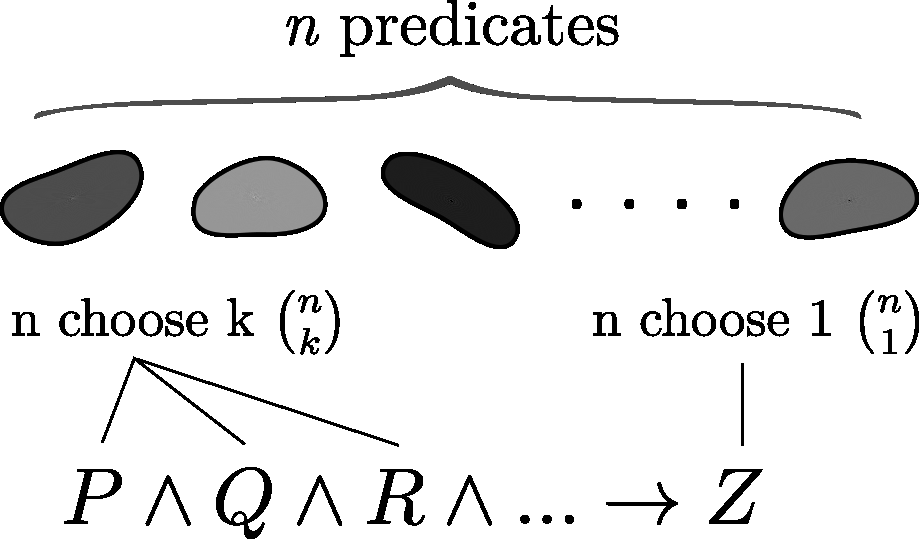
\includegraphics[scale=0.5]{geometric-logic-algorithm.png}}}
\end{equation}

\begin{itemize}
	\item What is a logic fact within a state?
	\item How does a rule generate a single new fact?
\end{itemize}

A fact consists of a point (in subject space) and a predicate that contains it.  The point itself does not suffice because it can belong to various predicates.

\subsection{How to determine if a rule is satisfied}

To apply a rule, each \textbf{atomic term} in the rule has to be satisfied.  For each predicate $Q()$, this is verified by testing if we have any points among the facts contained in $Q$.

If we have \textsf{father(john, pete)} as a fact then we certainly can satisfy \textsf{father}$(x,y)$.  But we already have the point \textsf{(john, pete)} which may satisfy other predicates $Q(x,y)$.  So our method is slightly more permissive (and thus more powerful) in rules matching.

How does the rule's RHS generate a new fact?  It should also be a (point, predicate) pair.  The point has to \textbf{match} the premise.  How could this be ensured?

Secondly, the output predicate may not cover the point.

The matching process:  Syntactically, we look at each literal in the rule and see if any fact unifies with the literal.  Geometrically, it means taking a point and checking if it lies inside a predicate.  If the fact is a (point, predicate) pair then it is certain that the point belongs to the predicate, so it is not necessary to check for membership.  The result is simply taking the point when the predicates match.  But we still need to keep track of which variables the point coordinates are binding to.

The matching of the second literal will also return a point, but its coordinates would be bound to different dimensions.

The binding of coordinates would be the basis of verifying the rule LHS.

RHS:  The bound variables (in various dimensions) need to be projected to the output space.  It may or may not be covered by the output predicate.  If not, the rule does \textit{not} apply.  This is in accord with the principle that rules should not change during inference.

\subsection{Handling variables in rules}

% Besides $(p, \gamma)$ we seem to need another parameter, the variable number specifying which of $\{ v_1, ..., v_n \}$ is referenced in a rule's argument.  This seems to be a parameter independent of $(p, \gamma)$.  But it seems irrelevant if there is no cylindrification?

Again drawing inspiration from Halmos' algebraic logic.  A monadic logic deals with predicates as $X \rightarrow \Omega$, whereas in polyadic logic one has $X^I \rightarrow \Omega$ where $I$ is an index set.  The elements of $I$ are \textbf{variables} even though they do not really change.  $X^I$ creates $I$ copies of the Subject Space $X$. Note that $(I \rightarrow X) \rightarrow \Omega$ is not isomorphic to $I \rightarrow (X \rightarrow \Omega)$.

% Solution:  Suppose we have a predicate of 2 arguments, eg. $\logic{loves}(\_, \_)$.  Train a neural network $P: X^I \rightarrow X^I$.  Train a ``selector'' function which chooses 2 out of $I$, in other words, a soft top-2 function $s: I \rightarrow \mathbb{R}$.  This gives a probability distribution over $I$, or more accurately speaking, a fuzzy-value distribution over $I$.  To evaluate a predicate $P$ at a point $(x,y)$, in other words to obtain the truth value of $P(x,y)$, we send $(x,y)$ to $P(x,y) \in X^I$.  Then the fuzzy values are applied to each copy of $X$ in $X^I$ such that...

For example $I = \{ 1,2,3,4 \}$ would provide 4 variables or ``slots'' for a rule to use.  A rule such as:
\begin{equation}
	\logic{father}(X_1,X_2) \wedge \logic{father}(X_2,X_3) \rightarrow \logic{grand\hbox{-}father}(X_1,X_3)
\end{equation}
uses 3 variables: $X_1, X_2, X_3$.  I have used the symbol $X$ with subscripts to denote variables, as a reminder that each variable is really a \textbf{copy} of our Subject Space $X$.

% The first predicate converges to dimensions $(\#1,\#2)$, the second predicate converges to dimensions $(\#2,\#3)$.  The output predicate converges to dimensions $(\#1,\#3)$.  These dimensions are discrete numbers and thus not differentiable.  To learn them by machine-learning, one way is to make them into stochastic actions and learn their probability distribution.

It is perhaps illuminating to rewrite the logic rule this way:
\begin{equation}
	\logic{father}(X^I) \wedge \logic{father}(X^I) \rightarrow \logic{grand\hbox{-}father}(X^I)
\end{equation}
where $I$ is at least $\{ 1,2,3 \}$.

In my mind, I had this mental picture:
\vspace{-0.2cm} \begin{equation}
\logic{father}(\begin{tikzpicture} \draw[line width=3pt, cyan!70] (0.2,0.9) -- (0.2,0) (0.5,0.9) -- (0.5,0) (0.8,0.2) -- (0.8,0); \draw[thick] (0,0) to (1,0); \end{tikzpicture})
\wedge
\logic{father}(\begin{tikzpicture} \draw[line width=3pt, cyan!70] (0.2,0.2) -- (0.2,0) (0.5,0.9) -- (0.5,0) (0.8,0.9) -- (0.8,0); \draw[thick] (0,0) to (1,0); \end{tikzpicture})
\rightarrow
\logic{grand\hbox{-}father}(\begin{tikzpicture} \draw[line width=3pt, cyan!70] (0.2,0.9) -- (0.2,0) (0.5,0.2) -- (0.5,0) (0.8,0.9) -- (0.8,0); \draw[thick] (0,0) to (1,0); \end{tikzpicture})
\end{equation}
where the blue bars represent some kind of relative ``proportion'' of variables, such that the overall construction could be \textbf{differentiable}.

% Each \textbf{argument} of a predicate would be associated with a \textbf{softmax} over the index set $I$, which selects one element out of $I$.  The softmax assigns, to each $i \in I$, a weight $w_i \in \mathbb{R}$.

% WRONG:  Then we can make copies of $X$ into $X^I$ as $\{ w_1 X_1, ..., w_n X_n \}$.  But this method assumes that the Subject Space $X$ has \textbf{vector space structure} and is amenable to scalar multiplication.  As I have argued in a blog article, the space of ``word embedding'' is actually a \textbf{metric space} rather than vector space.

% WRONG: A better solution is to associate the weight to that argument of the predicate such that the resulting \textbf{true value} of that predicate would be \textbf{weakened}.  The truth value of a predicate $P$ is evaluated by sending a point $(a,b)$ as input to a \textbf{neural network} representing $P$.  Its output is a real number normalized $\in [ 0,1 ]$ and interpreted as fuzzy truth-value.

The eventual implementation is quite natural:
\begin{align}
\nonumber
& \qquad \qquad \tikzmark{Y1}
\setlength{\fboxrule}{3pt}
\fcolorbox{cyan!70}{white}{$\hat{x}^1$}
\qquad
\tikzmark{Y2} \fcolorbox{cyan!70}{white}{$\hat{x}^2$}
\qquad
\tikzmark{Y3} \fcolorbox{cyan!70}{white}{$\hat{x}^3$} \\
& \qquad w_{ij}^k \\
& \nonumber \\
& \logic{father}(\tikzmark{X11} x_{11}, \tikzmark{X12} x_{12}, \tikzmark{X13} \Square_{13}) \wedge
\logic{father}(\tikzmark{X21} \Square_{21}, \tikzmark{X22} x_{22}, \tikzmark{X23} x_{23}) \rightarrow \logic{grand\hbox{-}father}(x_1,\Square_2,x_3)
\nonumber
\begin{tikzpicture}[remember picture,overlay]
\draw (pic cs:Y1) +(10pt,-7pt) -- ($ (pic cs:X11) +(7pt,12pt) $);
\draw (pic cs:Y1) +(10pt,-7pt) -- ($ (pic cs:X12) +(7pt,12pt) $);
\draw (pic cs:Y1) +(10pt,-7pt) -- ($ (pic cs:X13) +(7pt,12pt) $);
\draw (pic cs:Y1) +(10pt,-7pt) -- ($ (pic cs:X21) +(7pt,12pt) $);
\draw (pic cs:Y1) +(10pt,-7pt) -- ($ (pic cs:X22) +(7pt,12pt) $);
\draw (pic cs:Y1) +(10pt,-7pt) -- ($ (pic cs:X23) +(7pt,12pt) $);
\draw (pic cs:Y2) +(10pt,-7pt) -- ($ (pic cs:X11) +(7pt,12pt) $);
\draw (pic cs:Y2) +(10pt,-7pt) -- ($ (pic cs:X12) +(7pt,12pt) $);
\draw (pic cs:Y2) +(10pt,-7pt) -- ($ (pic cs:X13) +(7pt,12pt) $);
\draw (pic cs:Y2) +(10pt,-7pt) -- ($ (pic cs:X21) +(7pt,12pt) $);
\draw (pic cs:Y2) +(10pt,-7pt) -- ($ (pic cs:X22) +(7pt,12pt) $);
\draw (pic cs:Y2) +(10pt,-7pt) -- ($ (pic cs:X23) +(7pt,12pt) $);
\draw (pic cs:Y3) +(10pt,-7pt) -- ($ (pic cs:X11) +(7pt,12pt) $);
\draw (pic cs:Y3) +(10pt,-7pt) -- ($ (pic cs:X12) +(7pt,12pt) $);
\draw (pic cs:Y3) +(10pt,-7pt) -- ($ (pic cs:X13) +(7pt,12pt) $);
\draw (pic cs:Y3) +(10pt,-7pt) -- ($ (pic cs:X21) +(7pt,12pt) $);
\draw (pic cs:Y3) +(10pt,-7pt) -- ($ (pic cs:X22) +(7pt,12pt) $);
\draw (pic cs:Y3) +(10pt,-7pt) -- ($ (pic cs:X23) +(7pt,12pt) $);
\end{tikzpicture}
\end{align}
Each weight represents how ``strong'' an argument (lower row) occupies a variable slot (upper row).  \textbf{Softmax} normalizes the weights so that one of them would be most prominent, ie. the selected one.  Every argument can potentially appear in every variable slot, thus the bipartite graph is fully connected.

The resulting formula is this:  Each output slot $\hat{x}^k \in \hat{X}^I$ contains a \textbf{sum} of vectors from all arguments of all predicates on the left hand side of a rule:
\begin{equation}
\hat{x}^k \mathrel{:}= \underset{\text{predicates}}{\forall i \in} \; \underset{\text{arguments}}{\forall j \in} \left\langle \mathrm{soft}\max_{ij} w_{ij}^k \; , \; x_{ij} \right\rangle .
\end{equation}
Note that $ij$ is treated as one set of indices, so $x_{ij} = ( x_{11}, x_{12}, x_{13}, x_{21}, x_{22}, x_{23} )$ say, and $x_{ij}^\top$ is a simple column vector.

In the above method, the copying of a vector is not ``pure'' but may be contaminated by residuals of other vectors.  This is tolerable, as the vector embedding of tokens can allow for small perturbations.

The structure of our formula is reminiscent of the Transformer's \textbf{Self-Attention}:
\begin{equation}
\text{Attention}(\mathbf{Q,K,V}) = \text{soft}\max  \frac{\langle \mathbf{Q,K} \rangle}{\sqrt{d_k}} \mathbf{V}
\end{equation}
but softmax does not commute with inner products, so the two formulas are not equivalent.

What our formula does is to move variables around;  this suggests that the Transformer is also capable of moving \textbf{tokens} around.  The syntactic manipulation ability of Transformers has been corroborated by other researchers [cite].

For comparison, this is the \textbf{neural string diagram} for the traditional Self-Attention:
\begin{equation}
\vcenter{\hbox{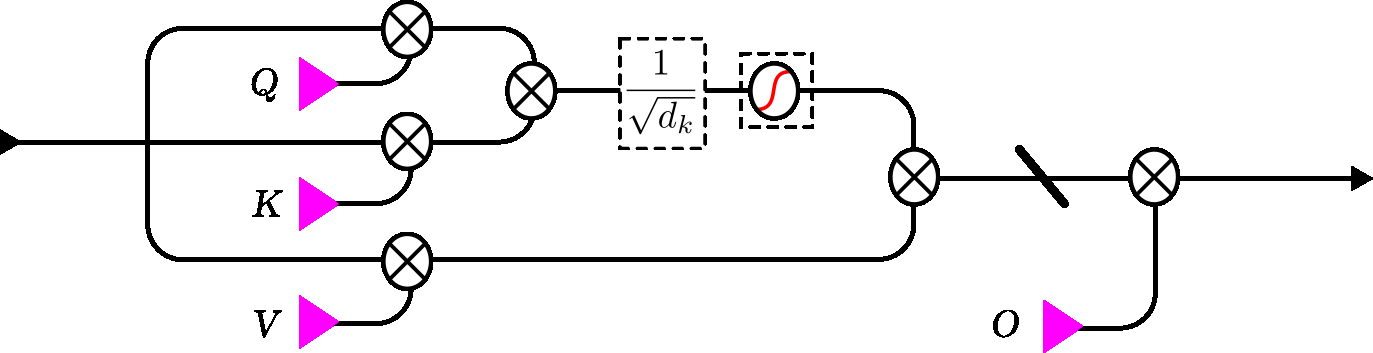
\includegraphics[scale=0.7]{Attention-string-diagram.png}}}
\end{equation}

The training of the neural network for predicate $P$ occurs in $X^2$ if the arity of the predicate is 2.  This has nothing to do with $X^I$ as the set $I$ of variables are only involved in logic rules.

To evaluate a rule:  Each predicate, such as $\logic{father(\_,\_)}$, is matched against some points, such as $(a,b)$.  The neural network returns a TV (truth value) independent of the variable space $X^I$.  But we need to put the point $(a,b)$ into $X^I$ via the \textbf{Softmax} selector.  This is repeated for all predicates on the LHS or ``head'' of the rule.  Then the truth values will determine if the rule is satisfied or not.  If yes, we will output a predicate such as $\logic{grand\hbox{-}father}(X_1, X_3)$.  Now we go back to $X^I$ to retrieve the point corresponding to the variables $(X_1, X_3)$.

\subsection{String diagram}

\begin{equation}
\hspace{-1.5cm}\vcenter{\hbox{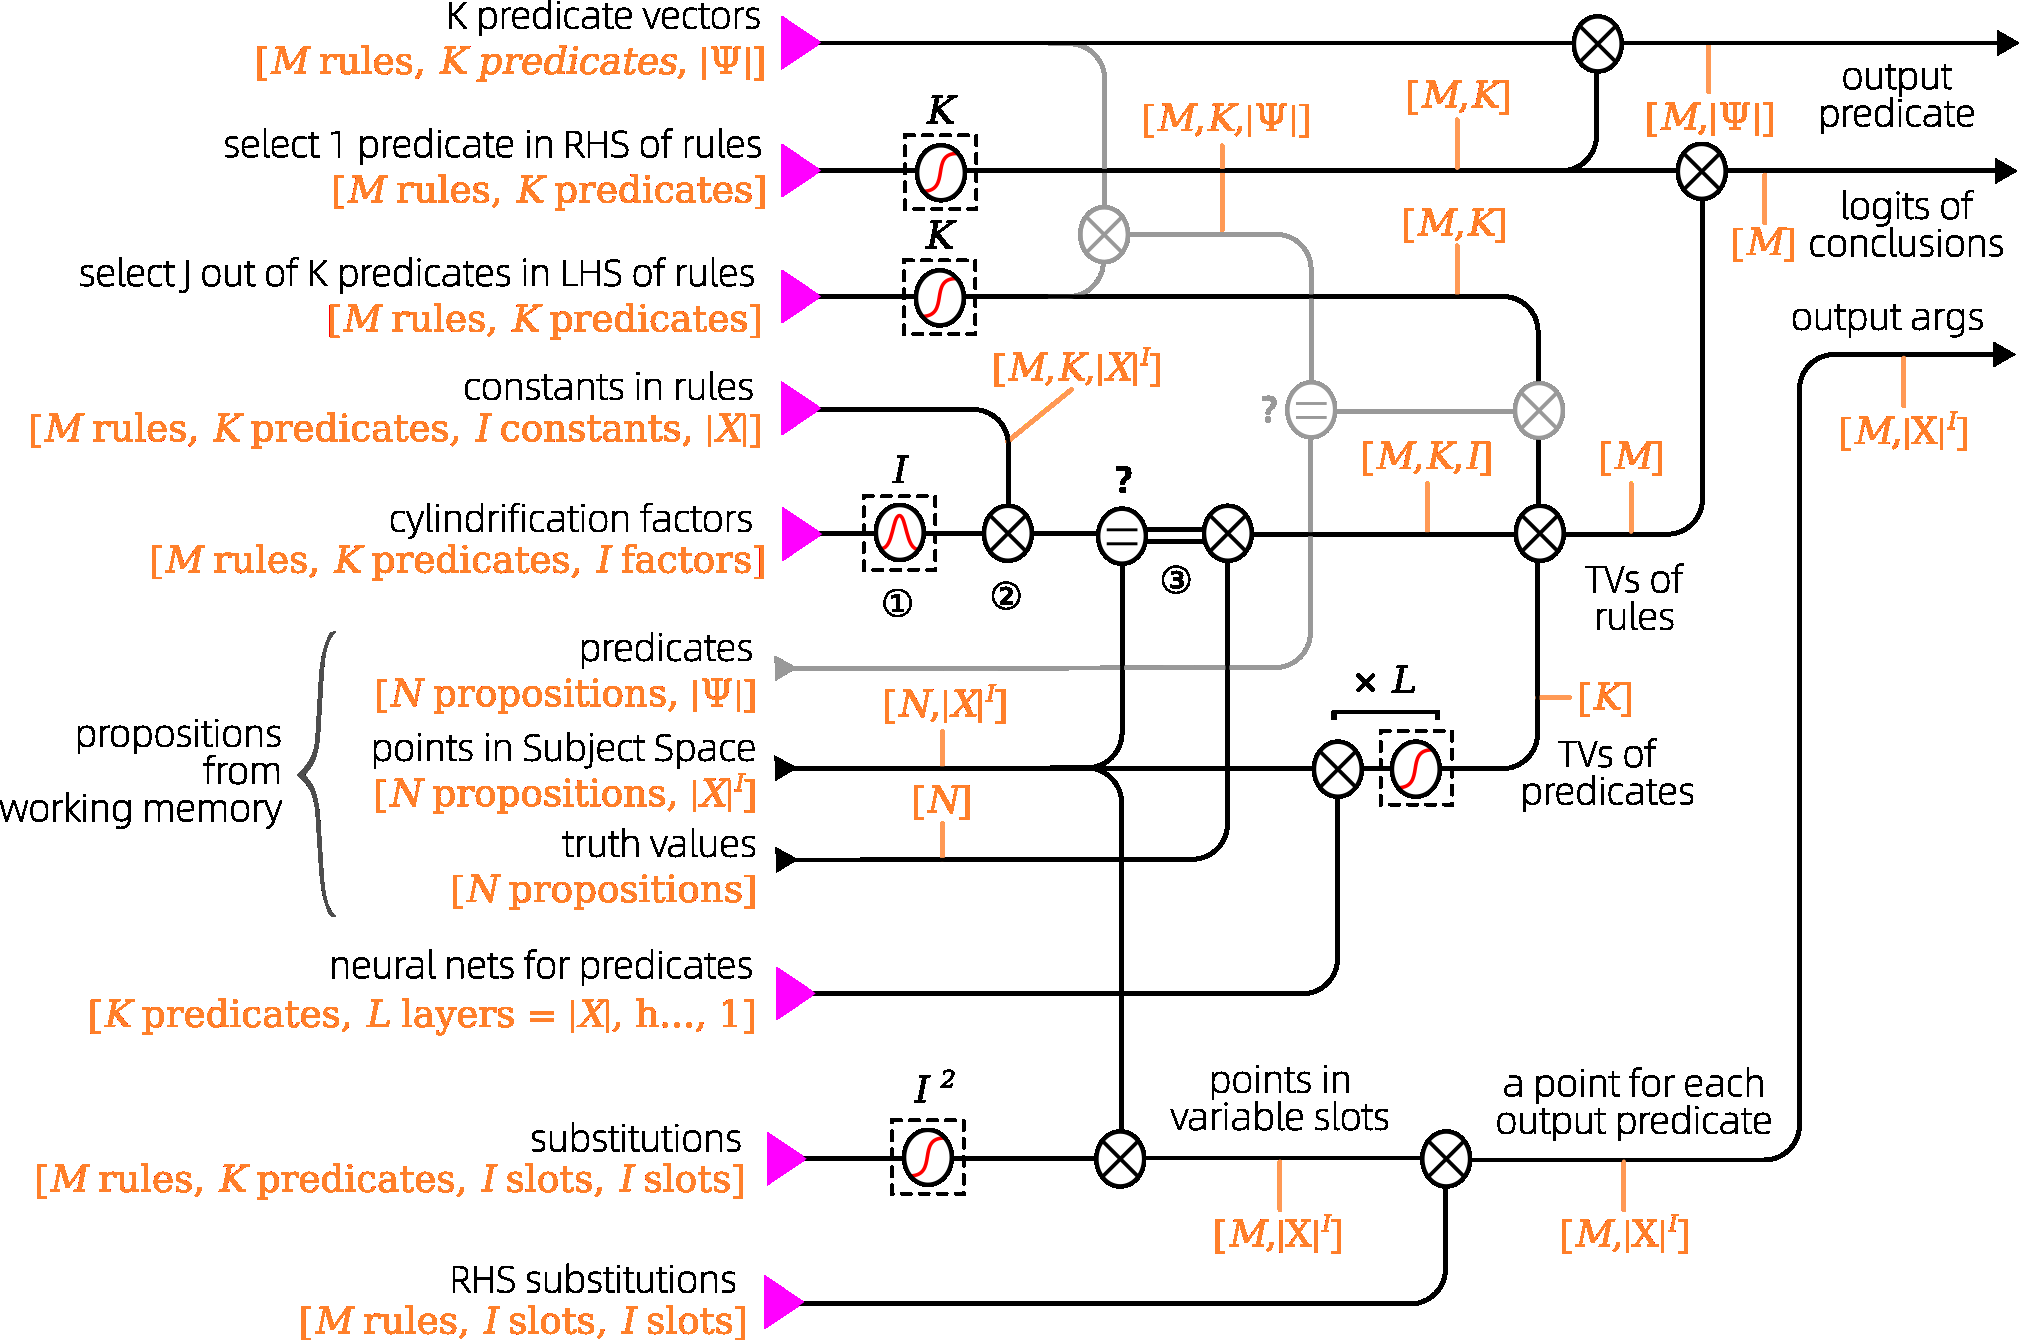
\includegraphics[scale=0.7]{logic-Transformer-string-diagram-2.png}}}
\end{equation}

\textbf{Legend:}
\begin{enumerate}
	\item The {\LARGE\color{magenta}\RIGHTarrow} indicates \textbf{internal data} supplied by the Transformer, similar to the Q,K,V matrices in traditional Transformers.  These are modified through ``learning'' or training.
	\item The 3 \RIGHTarrow's \ are \textbf{inputs} to the Transformer, this is matched with the 3 \textbf{outputs} on the right of the diagram.
	\item Tags {\color{orange}$[M,N,...]$} indicate the \textbf{dimensions} of data streams.
\end{enumerate}

\textbf{Remarks:}
\begin{enumerate}  % [label=\protect\circled{\arabic*}]
	\item[\textbullet] The \textbf{grayed-out} parts of the circuit tries to match the \textbf{predicates} of Working-Memory propositions to those in the rules.  For example, the predicate $\logic{loves}$ where $\logic{loves(John,Mary)}$ matches $\logic{loves}(X_1,X_2)$.  But I take the more liberal approach where matching succeeds whenever a point in Working Memory falls within the target predicate's region of definition, regardless of whether the source and target predicates match or not.  For example, assume $\logic{human(Socrates)}$ is in Working Memory, and we want to match against $\logic{mortal(X_1)}$.  This will succeed if the $\logic{human}$ region lies strictly within the $\logic{mortal}$ region in Subject Space.  If the predicate regions are learned properly, this would be the case.  Using this approach, rules are more easily satisfied, and the code seems to be simpler.

	\item[\circled{1}] We want to compare arguments of predicates in rules against propositions from Working Memory, ie, $\gamma(C) \stackrel{?}{=} c$, where $\gamma$ is a cylindrification factor (turned into a radial basis function), $C$ is a \textbf{constant} in a predicate in a rule, such as $\logic{Mary}$ in $\logic{loves}(\logic{John},\logic{Mary})$, to be matched against $c$, another constant argument of a predicate of a proposition from Working Memory.  In the above example, $(\logic{John},\logic{Mary})$ is a \textbf{point} in the Subject Space $X^2$.  $\logic{John}$ and $\logic{Mary}$ are also known as ``coordinates'' in $X^2$.

	\item[\circled{2}] On each step, we're not just comparing two elements, but two multi-dimensional matrices of elements.  On the left side is a matrix of dimensions $[M,K,|X|^I]$, for $M$ rules, each with $K$ predicates, each with $I$ argument slots, each containing an element of the Subject Space $X$.  On the right side (from Working Memory), we have a matrix of dimensions $[N,|X|^I]$, for $N$ propositions, each with $I$ argument slots, each containing an element of the Subject Space $X$. \\

	The operation $\stackrel{?}{=}$ is performed on the axis $I$, common to both sides.  For each rule $m \in M$, for each predicate $k \in K$, for each slot $i \in I$, we compare $C_{mki}$ against $c_{ni}$ for each proposition $n \in N$, for each argument slot $i \in I$.  This totals to $MKNI$ comparisons (the index $i$ counts only once).  This means trillions of comparisons, by our naive estimation of sizes.

	\item[\circled{3}] Each proposition in Working Memory has a truth value.  This TV has to be multiplied to the result in \circled{2}.
\end{enumerate}

The operation $a \stackrel{?}{=} b$ can be implemented by the function $(x \stackrel{?}{=} y) \coloneq y \cdot \sigmoid(x) + 1 - \sigmoid(x)$, where $\sigmoid$ is the sigmoid function such as $\frac{1}{1 + \exp(-100x + 50)}$.
\begin{equation}
\vcenter{\hbox{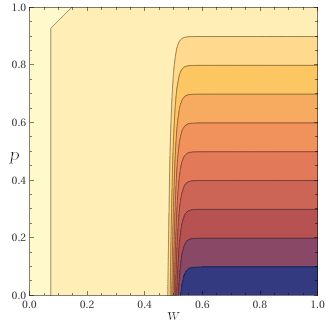
\includegraphics[scale=0.5]{selector-2D-plot.png}}}
\qquad
\vcenter{\hbox{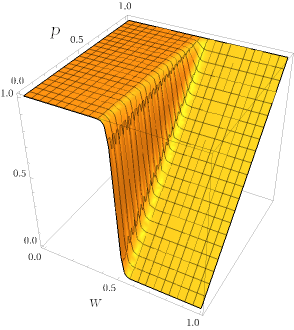
\includegraphics[scale=0.7]{selector-3D-plot.png}}}
\end{equation}

A trick often used in homotopy is: $h_t(x) = t \cdot f(x) + (1-t) \cdot g(x), t \in [0,1]$, so the function $h_t(x)$ is ``continuously deformed'' from $f(x)$ to $g(x)$.

We want to adjust the probability $p$ with weight $w$, such that
\begin{eqnarray}
\mbox{if } w = 0 \mbox{ or close to } 0, & \mbox{output } p = 1 \\
\mbox{if } w = 1 \mbox{ or close to } 1, & \mbox{output } p = p
\end{eqnarray}
Formula: output = $p \cdot t + 1 \cdot (1-t)$, this is the 'homotopy' trick where $t = \mbox{sigmoid}(w)$, specifically, $t = 1/(1 + \exp(-c \cdot (w - 0.5)))$ where $c$ is a scaling factor to make the sigmoid more steep and the sigmoid is shifted to where the midpoint occurs at w = 1/2.

\section{Computer representation of rules}

As explained in the Introduction (\S\ref{Ch0_logic_rules}), our rules are of the form:
\begin{equation}
\begin{aligned}
\mbox{rule 1:} & \quad \boxed{P^1_{1} X^1_{11}... X^1_{1I}} \;\wedge\; \boxed{P^1_2 X^1_{21} ... X^1_{2I}} \;\wedge\;...\; \boxed{P^1_K X^1_{K1} ... X^1_{KI}} \rightarrow \boxed{P^1_0 X^1_{01} ... X^1_{0I}} \\
\mbox{rule 2:} & \quad \boxed{P^2_{1} X^2_{11}... X^2_{1I}} \;\wedge\; \boxed{P^2_2 X^2_{21} ... X^2_{2I}} \;\wedge\;...\; \boxed{P^2_K X^2_{K1} ... X^2_{KI}} \rightarrow \boxed{P^2_0 X^2_{01} ... X^2_{0I}} \\
.... & \quad .... \\
\mbox{rule M:} & \quad \boxed{P^M_{1} X^M_{11}... X^M_{1I}} \;\wedge\; \boxed{P^M_2 X^M_{21} ... X^M_{2I}} \;\wedge\;...\; \boxed{P^M_K X^M_{K1} ... X^M_{KI}} \rightarrow \boxed{P^M_0 X^M_{01} ... X^M_{0I}}
	\raisetag{20pt}
\end{aligned}
\end{equation}

Each logic rule may vary in the following ways:
\begin{enumerate}
	\item number of literals and their polarity
	\item number of arguments
	\item each argument may be a logic variable or logic constant
	\item which specific logic variable or constant.
\end{enumerate}
The numbers in \#1 and \#2 can be fixed.

For \#3 and \#4, each variable or constant may be represented by a pair $(p, \gamma)$ where $p$ is a point (or coordinates) in the Subject Space, and $\gamma$ is the \textbf{cylindrification factor} representing the degree to which this argument is like a point or like a ``for all'' variable.  % But this is problematic as the dimension of the Subject Space $X$ is not the same as the dimension of the variable space $\{ X_1, X_2, ... , X_n \}$.

Each predicate has as its arguments $n$ copies of the Subject Space, ie, $X^n$.  One or more of the copies may be \textbf{cylindrified}.  The meaning of the cylindrical factor $\gamma$ is illustrated as follows:
%There are two senses of the word ``cylindrify.''  Think for example the change from (John, Mary) to ($x$, Mary) as in ``everyone loves Mary.''  In the first sense, the point John on the $x$-coordinate becomes ``everyone,'' ie, the entire $x$-dimension becomes a cylinder.  In the second sense, a cylinder appears on the $y$-axis at the position of Mary:
\begin{equation}
\vcenter{\hbox{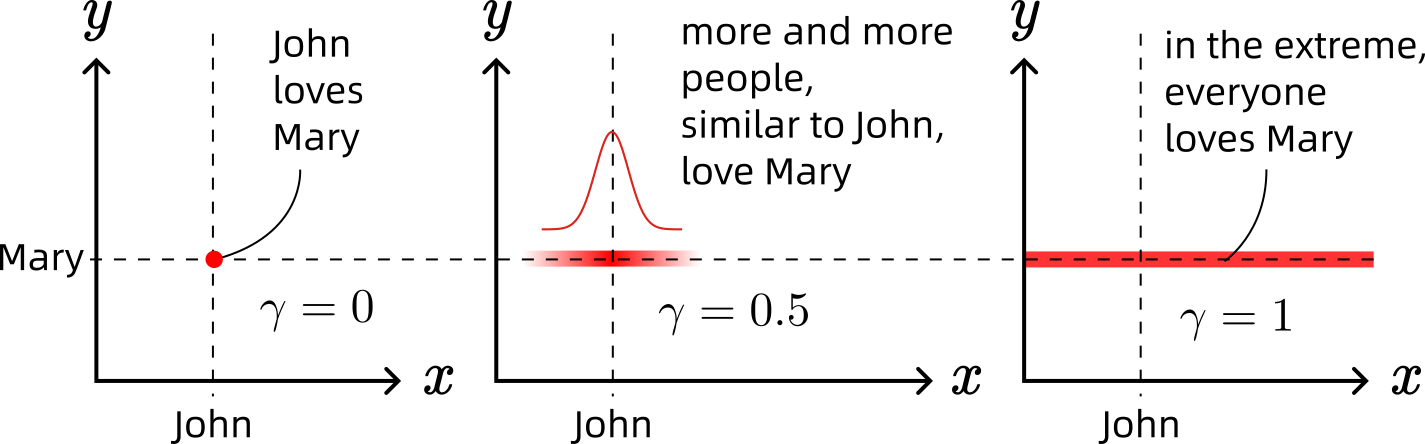
\includegraphics[scale=0.7]{cylindrify-example.png}}}
\end{equation}
In the above example, $(X,Y)$ are two copies of the Subject Space $X$, each is 1-dimensional.

During rule matching, suppose a point $p = (a,b)$ is presented from a proposition $P(p) = P(a,b)$ in the state $X$.  This is matched against a term $Q(X,Y)$ in the rule.  The rule-matching process seems costly, which suggests we may need to re-formulate a neural-network version of the \textbf{Rete algorithm} -- but such an algorithm would not be differentiable.  In fact, differentiability dictates that all rules must participate in matching at all times (or at least probabilistically with non-zero probabilities).

Anyway, the coordinate $a$ needs to be matched against the argument $X_1$, which may be a variable or a constant.  Denote the constant part of $X_1$ as $C_1$, so we try the matching $a \stackrel{?}{=} \gamma(C_1)$, where $\gamma$ is the cylindrification, a radial basis function.  This returns the truth value of the match.  At the same time, $a$ would be copied into the variable slot $X_1$ for substitution processing, independently.  This is OK, as the result will have a low TV if matching fails.

% The dimension $n$ is not just the number of variables appearing in one predicate in a rule, but the total number of variables appearing in a rule.

\vspace{1cm} \hrule \vspace{1cm}

We suggest the following values (for a general human-level intelligent agent):
\begin{equation}
\begin{tabular}{|c|c|c|}
	\hline
	\textbf{Meaning} & \textbf{Symbol} & \textbf{Est. typical values} \\
	\hline
	\# of rules & $M$ &  \sim millions \\
	\hline
	total \# of predicates & $K$ &  10,000's \\
	\hline
	\# of predicates per rule & $J$ &  2-10, typical 3,4 \\
	\hline
	\# of arguments per predicate & $I$ & 2, 3, 4  \\
	\hline
	Subject Space dimension & $|X|$ &  100-1000, typical 512, 768 \\
	\hline
	Predicate Space dimension & $|\Psi|$ &  same as above \\
	\hline
	Hidden layer size & $h$ & similar to $|X|$ \\
	\hline
	\# of propositions in working memory & $N$ & \sim 100 \\
	\hline
\end{tabular}
\end{equation}

Total number of parameters (in descending order of size) $= MKIX + MK\Psi + MKI^2 + MKI + 2MK + MI^2 + NIX + N\Psi + N + K(|X|+(L-2)h) \approx $ 20 trillion.  Perhaps $M$ and $K$ have to be reduced.

All the parameters (rules) of the Logic Transformer:
\begin{equation}
\begin{tabular}{|c|c|c|}
\hline
\textbf{Parameters} & \textbf{Dimensions} & \textbf{??} \\
\hline
$K$ predicates & $M$ rules, $K$ predicates, $|\Psi|$ & \\

\end{tabular}
\end{equation}

\section{``Higher-order'' logic}

The first-order Logic Transformer was simple to understand as a logic, but limited in expressive power as a logic.  As Ben Goertzel pointed out (during an online discussion with the author), it does not have mechanisms to handle \textbf{Skolem functions} and thus existential quantifiers.

One way to get around this problem is to define $\exists$ via a set of higher-order logic rules.  Without explicitly specifying how to do so (though I believe this can be done), we simply use a more powerful ``higher-order'' logic in the sense that rules admit substitutions in all (predicate or argument) positions, and hope that machine learning will learn the required axioms.

The new rules are of the form (without the special designation of ``predicates''):
\begin{equation}
\begin{aligned}
\mbox{rule 1:} & \quad \boxed{X^1_{11}... X^1_{1I}} \;\wedge\; \boxed{X^1_{21} ... X^1_{2I}} \;\wedge\;...\; \boxed{X^1_{K1} ... X^1_{KI}} \rightarrow \boxed{X^1_{01} ... X^1_{0I}} \\
\mbox{rule 2:} & \quad \boxed{X^2_{11}... X^2_{1I}} \;\wedge\; \boxed{X^2_{21} ... X^2_{2I}} \;\wedge\;...\; \boxed{X^2_{K1} ... X^2_{KI}} \rightarrow \boxed{X^2_{01} ... X^2_{0I}} \\
.... & \quad .... \\
\mbox{rule M:} & \quad \boxed{X^M_{11}... X^M_{1I}} \;\wedge\; \boxed{X^M_{21} ... X^M_{2I}} \;\wedge\;...\; \boxed{X^M_{K1} ... X^M_{KI}} \rightarrow \boxed{X^M_{01} ... X^M_{0I}}
\end{aligned}
\end{equation}

This gives us the revised string diagram:
\begin{equation}
\hspace{-1cm}\vcenter{\hbox{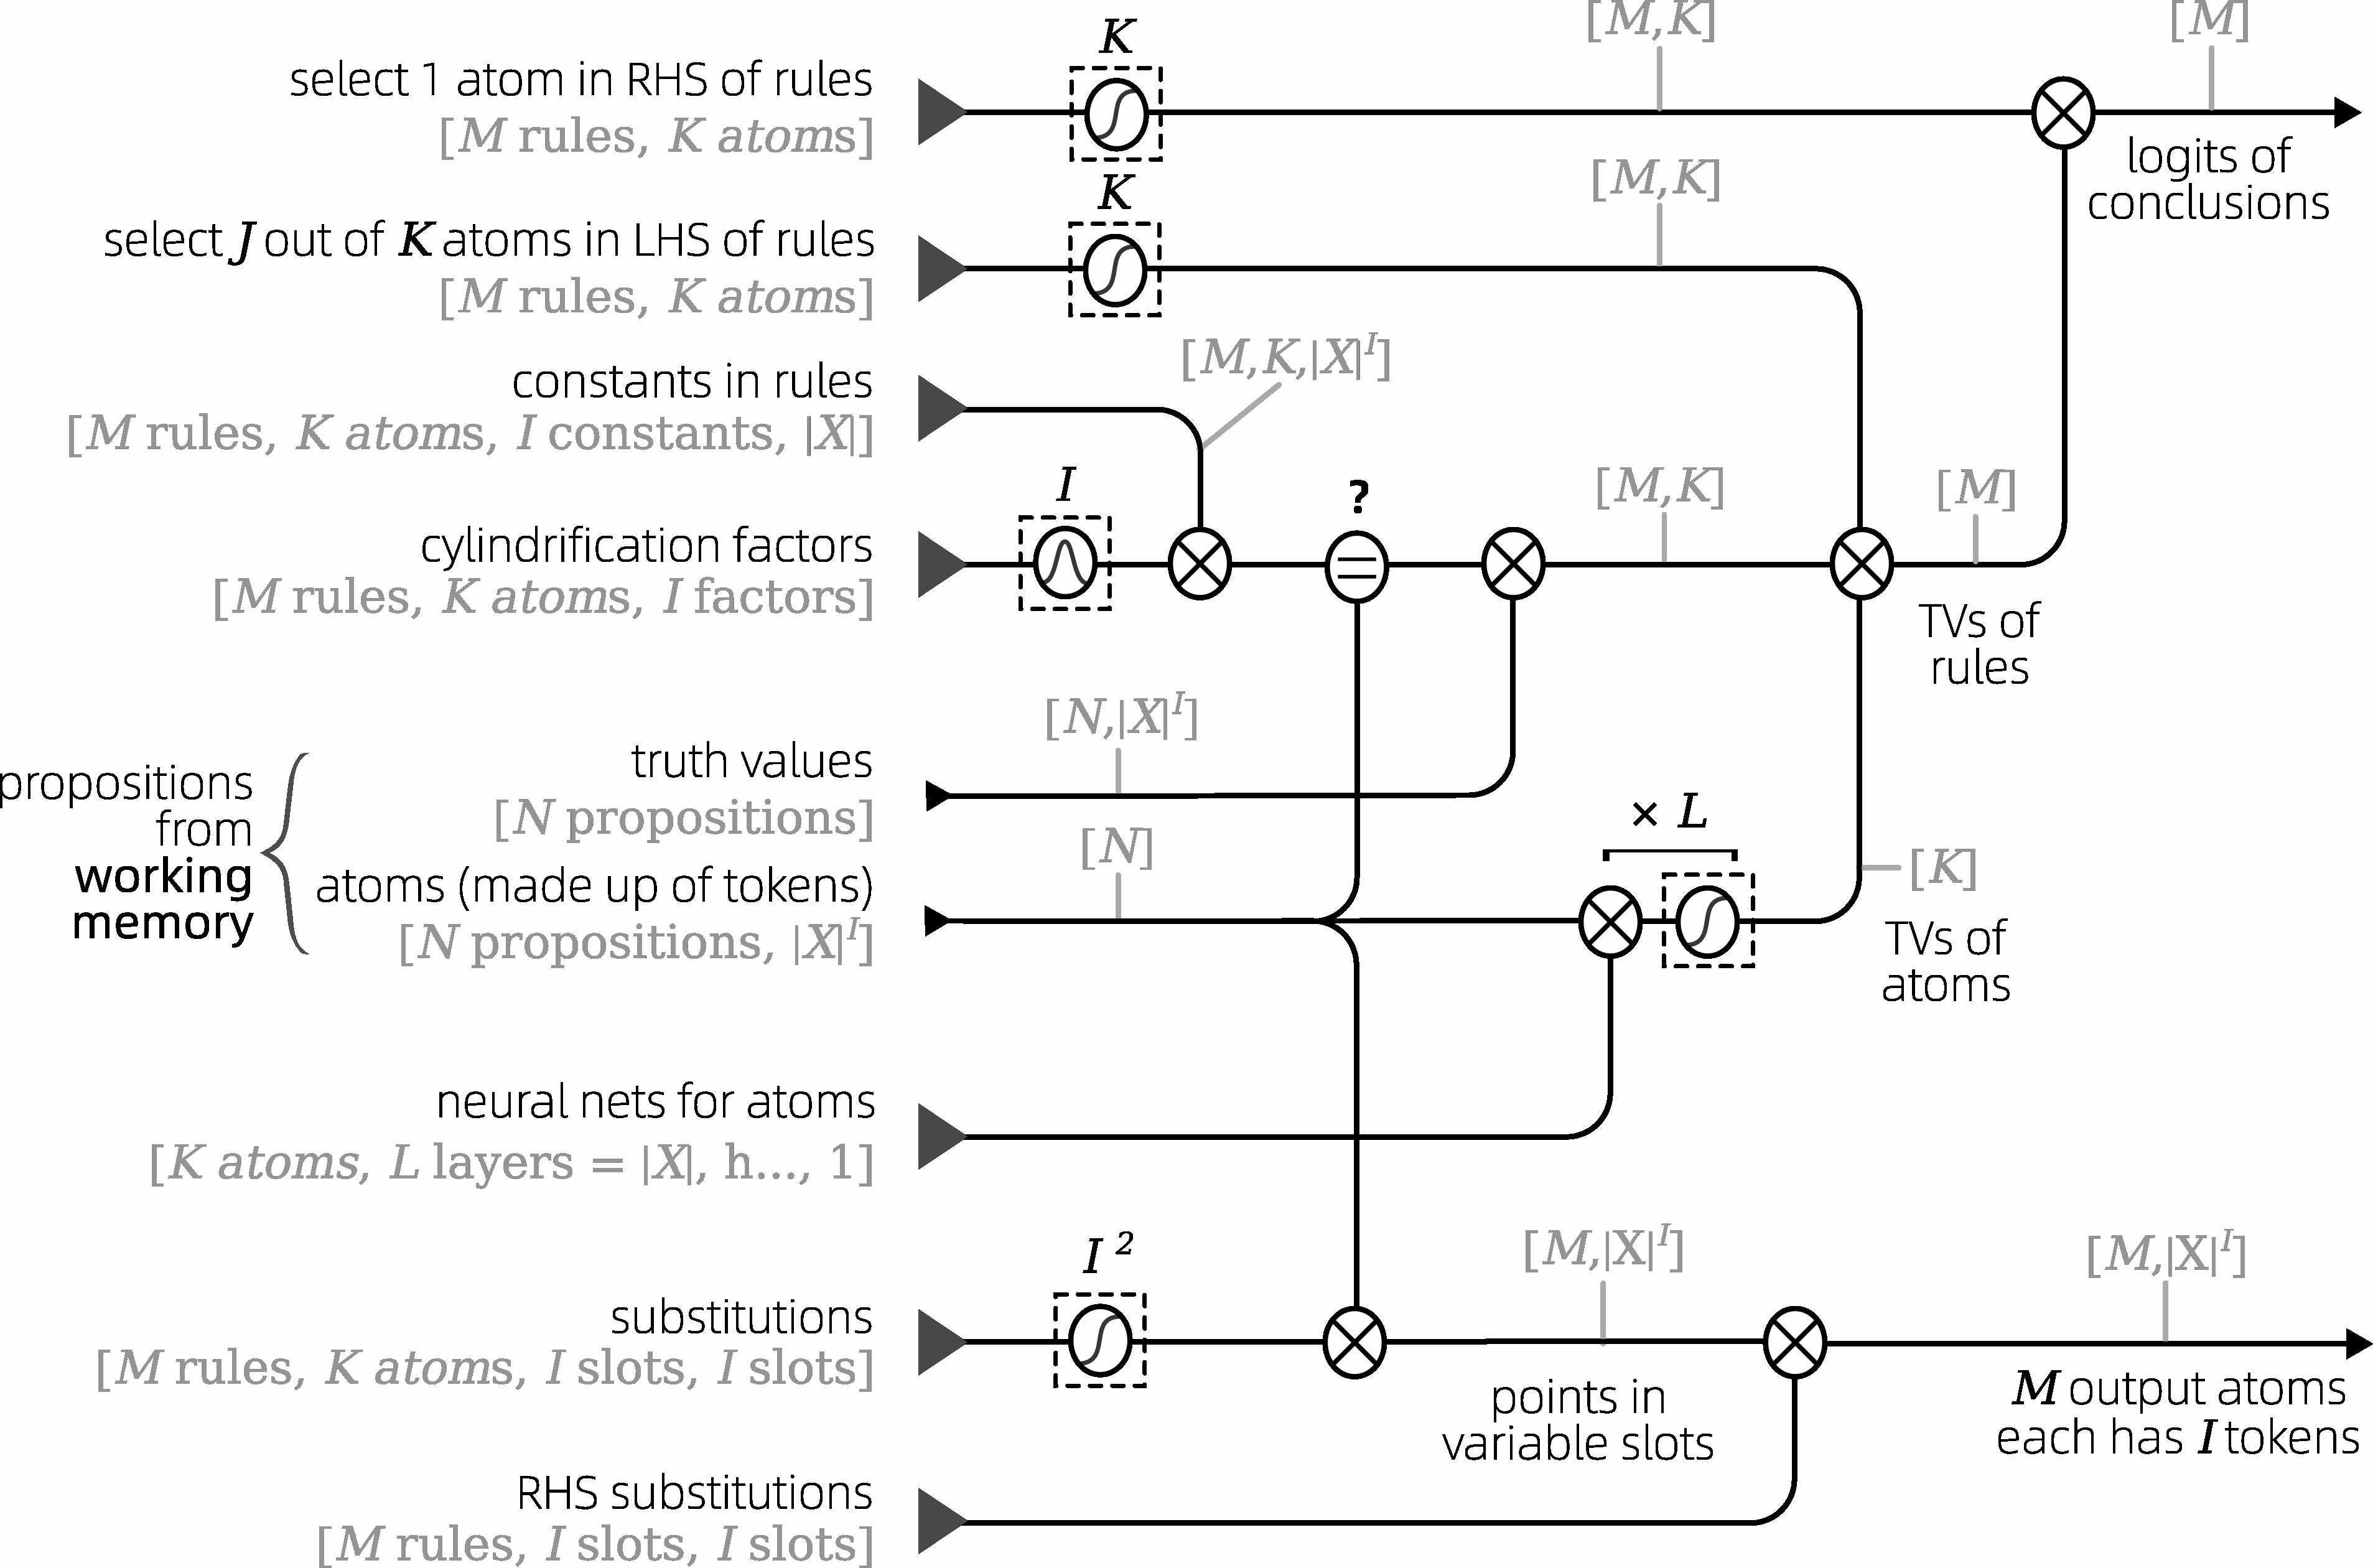
\includegraphics[scale=0.7]{logic-Transformer-string-diagram-3.png}}}
\end{equation}

\section{Rules recommender}

The rules recommender would be a set function:
\begin{equation}
\logic{Ru}: \{ \mbox{current state} \} \rightarrow \{ \mbox{set of rules} \}
\end{equation}
which has equivariant structure on both its input and output.  This suggests the \textbf{Transformer} architecture is suitable for learning this function.

But this is clearly \textbf{non-differentiable}!

\subsection{Differentiability}

In binary logic a rule either applies or does not apply.  To make the entire set of rules differentiable, rule application must be ``graded''.

So we propose a \textbf{probabilistic} rule-matching mechanism:
\begin{equation}
\vcenter{\hbox{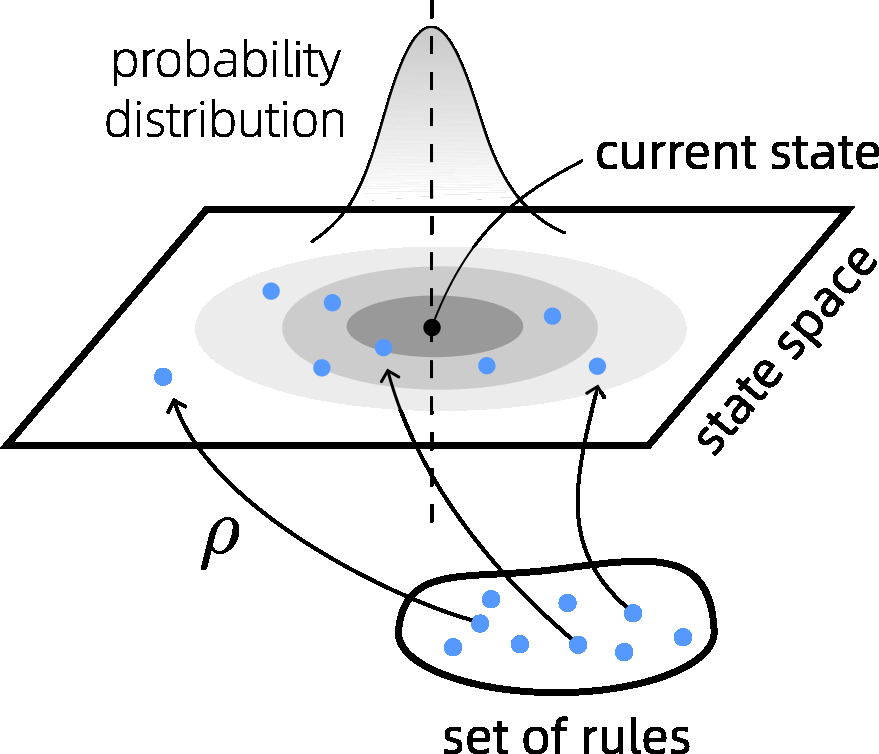
\includegraphics[scale=0.7]{rules-recommender.png}}}
\end{equation}
Rules are mapped by a function $\rho$ to the state space, such that rules are located close to the states they are most likely to match (this is a multi-objective optimization problem).  Given a current state $x$, denote the ball around it as $B(x, d)$.  The rules we predict most likely to match $x$ are given by $\rho^{-1}(B(x,d))$ for some distance $d$.  We can assign a Gaussian probability distribution centered around $x$ over such rules, so that rules are selected \textbf{probabilistically} for update.

It seems that doing so would not affect the convergence (of the learning algorithm) of the rules, but it would be much more efficient as the probability distribution is \textit{more} concentrated around $x$, so that large numbers of rules need \textit{not} be evaluated (for each state, at each time step).

% Rule 產生了新的結論,但先前選擇的 rule 是否影響新的 context?
% 其實 rules 本身可以分層。 最高的 rules 選擇下層的某些 rules。  但這只是其中一種做法。
% 其實如果有某 decision tree 負責 rules 的分流,似乎也仍然是可微的?
% but if the leafs of the decision tree are SHARED, differentiability may be a problem?
% the sorting tree can be deterministic... how does that affect differentiability?
% perhaps the rules at a whole can be regarded as a single function transforming the current state to the next state.  Differentiability would be discussed with respect to this function.
% What does it mean for differentiability to be broken...?  The total rule function must change infinitesimally per each update...
% differentiation is like dy/dx.... when x = the total function...  the question is whether we can always perform x+dx... where dx will not be of finite length
% the state x will change from step to step....  but that's not a problem...  we care about the

\begin{equation}
x_{t+1} = \squareF(x_t; \Theta)
\end{equation}
where $\Theta$ are all the parameters that determine the rules, $\squareF$ is the total function aggregating all the rules.  If we vary any one rule parameter, does it change abruptly?  The parameters $\Theta$ include the rules-sorting function $\rho$.

For gradient descent we need to calculate $\nabla_\Theta \mathcal{L}$ where $\Theta$ are all the parameters of rules, and the loss function is defined as the sum of errors over all rules, $\displaystyle \mathcal{L} = \sum_{\text{all rules}} \epsilon^2 $.  Each error usually is given by the difference as compared against a reference value (supervised learning), but in our case such a value is unavailable, instead the objective comes from reinforcement learning, ie, the Hamilton-Jacobi-Bellman equation:  $\displaystyle J(x_{t+1}) = \max_a [ \gamma J(x_t) + R(x_t,a) ] $, where $a$ means \textbf{action}.  In the logic-based setting, an action means applying a logic rule to change the state.

Policy function:
\begin{equation}
\pi: X \times A \rightarrow [0,1]
\end{equation}
By the \textbf{Policy Gradient Theorem}, calculation of $\nabla_\Theta J$ translates to calculating $\nabla_\Theta \pi$.

In reinforcement learning, in particular the \textbf{Policy Gradient} algorithm, we need to calculate the gradient $\nabla_\phi \mathcal{L}(\phi)$ of a loss function of the form:
\begin{equation}
\mathcal{L}(\phi) = \mathbb{E}_{z \sim q_\phi(z)}[ f(z) ] .
\end{equation}
The expectation gives an integral $\displaystyle \nabla_\phi \mathcal{L}(\phi) = \nabla_\phi \int dz q_\phi(z) f(z)$ which removes the ``randomness'' and evaluates to a real number.  This allows to be handled by traditional differential calculus.

At each state, the application of all rules results in a list of all available actions.  The differentiability problem may arise from probabilistic rule-matching.

\section{Interestingness}

This can be implemented implicitly by making the inference algorithm output a probability distribution over all deduced conclusions and then picking the most probable one.

\section{Combining logic and reinforcement learning}

\subsection{Logical policy function}

The policy function $\pi: X \times A \rightarrow [0,1]$ should be implemented with logic structure.  The current state would be matched against rules selected by the rules recommender, and then each rule would be applied, resulting in conclusions $Z_i$ each associated with a probabilistic strength $\mathbb{P}(Z_i)$.  These are the available actions and their probabilities as given by the policy.

\vspace{1cm} \hrule \vspace{1cm}

This section concerns how to establish the ``link'' from logic to reinforcement learning.

For reinforcement learning, I find it easier to consider Q-learning, ie, learning the utility function $Q(s,a)$, where $s$ = current state and $a$ = action taken in current state.

During forward inference, each logic rule of the form (also known as Horn form):
\begin{equation}
	P \wedge Q \wedge R \wedge ... \rightarrow Z
\end{equation}
yields a conclusion $Z$.  But the ``truths'' of the premises $P,Q,R,..$ are not binary but fuzzy, because the rules have to be differentiable (this can be implemented by softmax).  Thus each conclusion $Z$ is also fuzzy.  The application of all the rules yields a set of conclusions $\{ Z_i \}$, with their associated fuzzy truth values, which we can normalize as a probability distribution over all available next actions.  This can be regarded as the \textbf{policy function} $\pi(a|s)$, which gives the probability of an action given the current state, $\mathbb{P}(a|s)$.

In Q-learning we need to learn the values $Q(s,a)$.  Given the reward $R$, $Q(s,a)$ satisfies the Bellman equation:
\begin{equation}
	Q(s,a) \mathrel{+}= \eta \big( R + \gamma \max_{a'} Q(s',a') - Q(s,a) \big)
\end{equation}
where $\eta$ is the learning rate, $\gamma$ is the discount rate of values.

The policy function $\pi(a|s)$ is not exactly the same as $Q(s,a)$, but there is a trick that can relate them, that is the basis of \textbf{Soft-Q learning} (Soft Actor-Critic, SAC):
\begin{equation}
	\pi(a|s) \propto \exp Q(s,a)
\end{equation}

The situation can be illustrated by the following figure (not a commutative diagram):
\begin{equation}
\begin{tikzcd}[column sep=1.5cm, row sep=0.6cm]
	{} & {} & \parbox{1.5cm}{\linespread{-0.5}\selectfont\centering Bellman update} \arrow[d] \\
	\parbox{1.2cm}{\linespread{-0.5}\selectfont\centering logic rules} \arrow[r]
	& \pi(a|s) \arrow[r,shift left=2pt,harpoon,"\log"]
	& Q(s,a) \arrow[l, shift left=2pt, harpoon, "\exp"]
\end{tikzcd}
\end{equation}
Logic rules give us $\pi(a|s)$, which in turn gives us $Q(s,a)$, but $Q(s,a)$ is also determined by Bellman update.

My solution is:  Logic outputs a finite set of actions, to each action is associated a weight, which we identify as $Q$.  Use Bellman update to train these $Q$ values.  To choose an action, calculate $\pi(a|s)$ as suggested by the Soft-Q method.  This has the effect of \textbf{maximum-entropy} exploration.

\section{Basics of DQN (Deep Q Learning)}

The \textbf{Bellman optimality condition} says that:
\begin{equation}
	Q^*_t = \max_{a} \{ R + \gamma Q^*_{t+1} \}
\end{equation}
where $()^*$ denotes optimal values.

In the \textbf{Bellman update},
\begin{equation}
	Q_t \mathrel{+}= \eta \cdot \mbox{TD-error}
\end{equation}
where TD = \textbf{temporal difference} is defined as:
\begin{equation}
	\mbox{TD-error} = \overbrace{R + \gamma \max_{a'} Q(s_{t+1},a')}^{\mbox{ideal value}} \overbrace{ - \; Q(s,a)}^{\mbox{current value}} .
\end{equation}
So obviously the Bellman update causes the current value of $Q$ to \textbf{converge} to that of the optimal value $Q^*$.

Remember that, in the simplest \textbf{Q-table} method, we apply the Bellman update over Q-table entries.  The \textbf{DQN} approach differs in that, instead of a Q-table, we use a deep neural network in its place.  So the updating of the Q-table now becomes updating the DQN via \textbf{gradient descent}.

\chapter{Combining RL and Auto-regression}
\label{chap:RL-Autoregression}

	% Combining RL and Autoregression
\chapter{Experiments}\label{chap:Experiments}

\section{Representation of states and rules}

At any time the state is a set of facts, ie, pairs of (point $\in$ predicate).

There will be $K$ predicates and $M$ rules.

Each rule is a conjunction of all predicates.  If $K$ is large, the rules would be cumbersome.

Having a large number of rules, $M$, seems not to have a deleterious effect, if the rules recommender is good at its job.

Each literal in the rule may be negated, how to handle this?

Each literal contains a predicate and its arguments, which can be constants or variables.

It seems that genetic algorithms would be best suited for this kind of search for rules...  or unless the rules are represented in such a way that they can continuously vary in a differentiable manifold.

For TicTacToe, let's say number of rules = 50.


\chapter{Conclusions}\label{chap:conclusions}

Some conclusion text.


%% -------------------------------------------------
%% References
%% -------------------------------------------------

\printbibliography[heading=bibintoc,title=References]

%% -------------------------------------------------
%% Appendices
%% -------------------------------------------------
\appendix

\chapter{List of Publications}
% "List of Publications" citations can be stored in `mythesis.bib` or,
% another bib file, remember to add its name in `\addbibresource{}`

% Journal Publications
\paperlist[Journal Publications]{ChaiACSNano2022,HermanNature2007,WarrenSci.Adv.2022}

% Conference Publications
\paperlist[Conference Publications]{LuConf.LasersElectro-Opt.2021Pap.SW3B12021, JehleImagingAppl.Opt.20162016Pap.IM4F22016}

% You can add customized title name in the []

\chapter{FYTGS Requirements}
\label{chap:thesis-preparation}

The requirements are from the \href{https://rpghandbook.hkust.edu.hk/appendices-guidelines-on-thesis-preparation}{RPG Handbook}.

\section{Components}

\subsection{Order}

A thesis should contain the following parts in the order shown:

\begin{enumerate}
  \item Title page, containing in this order:
        \begin{enumerate}
          \item Thesis title
          \item Full name of the candidate
          \item Degree for which the thesis is submitted
          \item Name of the University, \emph{i.e.} The Hong Kong University of Science and Technology
          \item Month and year of submission
        \end{enumerate}
  \item Authorization page
  \item Signature page
  \item Acknowledgments
  \item Table of contents
  \item Lists of figures and tables
  \item Abstract ($\leq$ 300 words.)
  \item Thesis body
  \item Bibliography
  \item Appendices and other addenda, if any.
\end{enumerate}

\subsection{Authorization page}

On this page, students authorize the University to lend or reproduce the thesis.

\begin{enumerate}
  \item The copyright of the thesis as a literary work vests in its author (the student).
  \item The authorization gives HKUST Library a non-exclusive right to make it available for scholarly research.
\end{enumerate}

\subsection{Signature page}

This page provides signatures of the thesis supervisor(s) and Department Head confirming that the thesis is satisfactory.

\subsection{Acknowledgments}

The student is required to declare, in this section, the extent to which assistance has been given by his/her faculty and staff, fellow students, external bodies or others in the collection of materials and data, the design and construction of apparatus, the performance of experiments, the analysis of data, and the preparation of the thesis (including editorial help). In addition, it is appropriate to recognize the supervision and advice given by the thesis supervisor(s) and members of TSC.

\subsection{Abstract}

Every copy of the thesis must have an English abstract, being a concise summary of the thesis, in 300 words or less.

\subsection{Bibliography}

The list of sources and references used should be presented in a standard format appropriate to the discipline; formatting should be consistent throughout.

\textbf{Sample pages} of both MPhil and PhD theses are provided here (MPhil / PhD), with specific instructions for formatting page content (centering, spacing, etc.).

\section{Language, Style and Format}

\subsection{Language}

Theses should be written in English.

Students in the School of Humanities and Social Science who are pursuing research work in the areas of Chinese Studies, and who can demonstrate a need to use Chinese to write their theses should seek prior approval from the School via their thesis supervisor and the divisional head.

If approval is granted, students are also required to produce a translation of the title page, authorization page, signature page, table of contents and the abstract in English.

\subsection{Pagination}

\begin{enumerate}
  \item All pages, starting with the Title page should be numbered.
  \item All page numbers should be centered, at the bottom of each page.
  \item Page numbers of materials preceding the body of the text should be in small Roman numerals.
  \item Page numbers of the text, beginning with the first page of the first chapter and continuing through the bibliography, including any pages with tables, maps, figures, photographs, etc., and any subsequent appendices, should be in Arabic numerals.
  \item Start a new page after each chapter or section but not after a sub-section.
\end{enumerate}

\emph{Note: That means the Title page will be page i; the first page of the first chapter will be page 1.}

\subsection{Format}

\begin{enumerate}
  \item A conventional font, size 12-point, 10 to 12 characters per inch must be used.
  \item One-and-a-half line spacing should be used throughout the thesis, except for abstracts, indented quotations or footnotes where single line spacing may be used.
  \item All margins—top, bottom, sides—should be consistently 25mm (or no more than 30mm) in width. The same margin should be used throughout a thesis. Exceptionally, margins of a different size may be used when the nature of the thesis requires it.
\end{enumerate}

\subsection{Footnotes}

\begin{enumerate}
  \item Footnotes may be placed at the bottom of the page, at the end of each chapter or after the end of the thesis body.
  \item Like references, footnotes should be presented in a standard format appropriate to the discipline.
  \item Both the position and format of footnotes should be consistent throughout the thesis.
\end{enumerate}

\subsection{Appendices}

The format of each appended item should be consistent with the nature of that item, whether text, diagram, figure, etc., and should follow the guidelines for that item as listed here.

\subsection{Figures, Tables and Illustrations}

Figures, tables, graphs, etc., should be positioned according to the scientific publication conventions of the discipline, e.g., interspersed in text or collected at the end of chapters. Charts, graphs, maps, and tables that are larger than a standard page should be provided as appendices.

\subsection{Photographs/Images}

\begin{enumerate}
  \item High contrast photos should be used because they reproduce well. Photographs with a glossy finish and those with dark backgrounds should be avoided.
  \item Images should be dense enough to provide 300 ppi for printing and 72 dpi for viewing.
\end{enumerate}

\subsection{Additional Materials}

Raw files, datasets, media files, and high resolution photographs/images of any format can be included.

\emph{Note: Students should get approval from their department head before deviating from any of the above requirements concerning paper size, font, margins, etc. }


\end{document}
